\pagestyle{fancy}

\graphicspath{ {Figures/Chapter6_EmissivityMeasurement/} }

In chapter \ref{ch:TempModeling}, we saw that material properties such as melting (or sublimating) temperatures, heat capacity, thermal conductivity, emissivity, etc. play a very important role in properly describing the thermal behavior and limitations of our detectors. Uncertainties in these values yielded uncertainties in the final simulated results. The highest material parameter uncertainty was found in the case of the tungsten emissivity, showing an average uncertainty of around $43.26 \%$.

Figure \ref{fig:EmissUnc} tries to break down this uncertainty value in more detail. In this figure, every curve represents the emissivity value (as a function of the temperature) reported by a different source. A summary of all these sources and their corresponding reference can be found in \parencite[]{ref:MatProperties}. From this figure we can observe the big spread of the emissivity value reported by the different sources, covering almost all the available ranges (0 - 1). 

\begin{figure}[h]
    \centering
    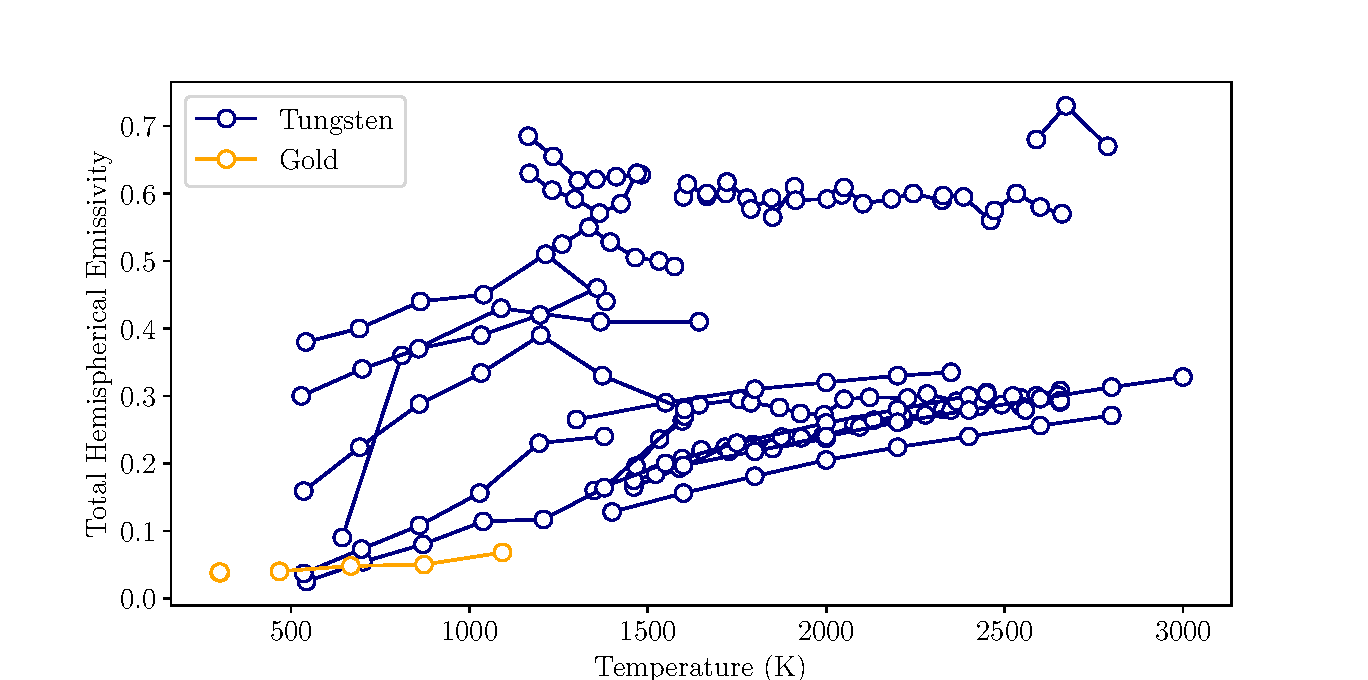
\includegraphics[width=0.80\columnwidth]{EmissivityLiteratureVar/EmissivityLit.pdf}
    \caption{Examples of total emissivity measurements for Gold and Tungsten. From \parencite[][]{ref:MatProperties}}
    \label{fig:EmissUnc}
\end{figure}

At CERN, in particular, at LINAC4, SEM grid detectors are made of gold-coated tungsten wires. Emissivity is a surface property, so the emissivity of gold should be considered. However, as previously shown, due to the high temperatures reached by the detectors, gold can be evaporated from the surface. This arises an extra uncertainty when choosing the correct value for this parameter. 

For these reasons, we decided it was necessary to experimentally measure the emissivity of the wires that are being used in the SEM grids, so more accurate thermal limits can be calculated. In this chapter, we will explain in more detail the concept of emissivity, we will introduce some commonly used methods for measuring this property and we will explain why the calorimetric method was chosen. This will be followed by a detailed explanation of the experimental setup and the numerical algorithms employed for determining the values of the emissivity.

\section{Essentials in radiometry}

A good starting point for this discussion is introducing the concept of the black body, which is crucial for understanding the concepts of heat radiation and its laws. This concept was first introduced in 1860 when Gustav r. Kirchoff \parencite[][]{ref:Kirchoff}. It describes an idealized physical body that allows all incident radiation to pass into it (no reflected energy) and internally absorbs all the incident radiation (no energy transmitted through the body), for all radiations and angles of incidence. For this ideal black body, in thermal equilibrium, the body emits all the absorbed energy. In 1900 Max Plank formulated a mathematical relationship to explain the spectral-energy distribution emitted by a black-body \parencite[][]{ref:Planck}:

\begin{equation}
    B_{0}\left(\lambda,T\right) = \frac{2hc^2}{\lambda^5}\frac{1}{e^{\frac{hc}{\lambda k_B T}}-1}
    \label{eq:plank}
\end{equation}

B refers to the spectral emissive power per unit area, and it is expressed in units of ($W\cdot sr^{-1} \cdot m^{-3}$). h is Plank's constant ($h = 6.62617\cdot 10^{-34}$ Js) and $K_b$ is Boltzmann's constant ($K_{B} = 1.38066\cdot 10^{-23}$ J/K). Plank radiation has a maximum intensity at a wavelength that depends on the temperature of the body, see figure \ref{fig:MaxWavelenght}. For room temperature (300K), a body emits thermal radiation that is mostly infrared. At higher temperatures, the peak of radiation moves towards the visible range, and we can see the body glowing visibly read. If the body were able to withstand temperatures around 5000K we could see it become bright yellow or blue-white, and it would emit a high amount of ultraviolet light and even x-rays. 

\begin{figure}[h]
    \centering
    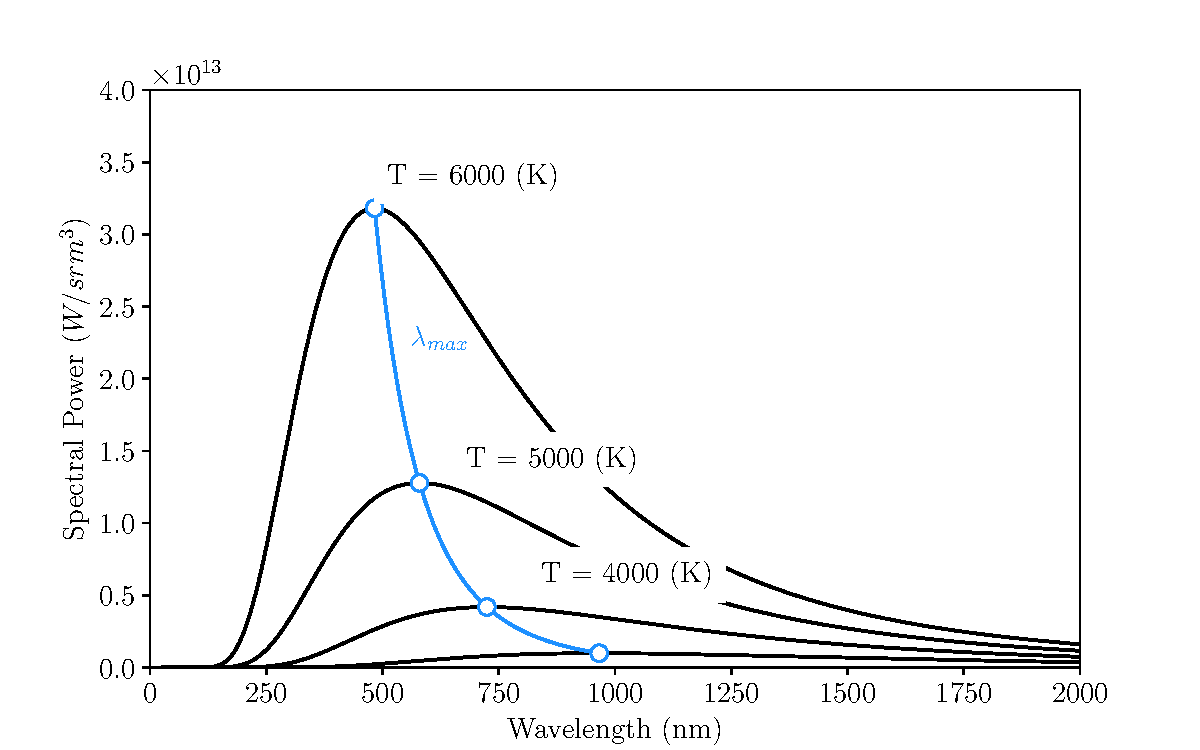
\includegraphics[width=0.80\columnwidth]{PlankEquation/PlankEq.pdf}
    \caption{Black body spectrum for different temperatures. Blue line, Wien's displacement law.}
    \label{fig:MaxWavelenght}
\end{figure}

The maximum wavelength for a given temperature can be calculated with Wien's displacement law:

\begin{equation}
    \lambda_{max} = \frac{0.2898}{T}
\end{equation}

Here $\lambda_{max}$ is given in (cm). If one is interested in the total power emitted per unit area at a given temperature, equation \ref{eq:plank} can be integrated over all frequencies and solid angles. This is described by Stefan-Boltzmann law, which can be written as: 

\begin{equation}
    P = \sigma T^4
\end{equation}

With $\sigma = 5.67044\cdot 10^{-8}$ ($W m^{-2} K^{-4}$). In practice, only very few objects approach the absorbing properties of an ideal black body. Even if that is the case, the concepts that we just introduced, are an important standard of comparison for the emitting and absorbing characteristics of real objects \parencite[][]{ref:Usefulbook}. Usually, the treatment of radiation emission from real bodies is done using a parameter called emissivity, which compares the radiation emitted from the real body with the radiation emitted from an ideal black body at the same temperature. This parameter can be defined as follows:

\begin{equation}
    Emissivity \hspace{0.1cm} (\epsilon) = \frac{Radiant \hspace{0.1cm}  Power }{Radiant \hspace{0.1cm}  Power \hspace{0.1cm} Black\hspace{0.1cm}  Body}
\end{equation}

This parameter takes values between 0 and 1. The closer this parameter is to 1, the closer the body radiates as an ideal black body. More specifically, the emissivity can have different values depending on whether or not one distinguishes the radiation of the surface is emitted on a given wavelength, in a particular direction or at a given temperature, $\epsilon = \epsilon(\lambda , T, \theta, \phi)$.

Figure \ref{fig:EmissSche} shows a schematic description of the emissivity definitions depending on their dependencies. Different names are given to the different values of emissivity. 


\begin{itemize}
    \item \textbf{Directional Monochromatic (or Spectral) Emissivity: } Is the ratio between the spectral radiance of a body and that of the black body for a given direction and wavelength:
    \begin{equation}
        \epsilon_{\lambda,\theta,\phi}\left(\lambda,T,\theta,\phi\right) = \frac{B_{Material}\left(\lambda,T,\theta,\phi\right)}{B_{0}\left(\lambda,T\right)}
    \end{equation}
    This is the finest description for a given material. $B_0$ does not depend on the incidence for a black body. 
    \item \textbf{Hemispherical Monochromatic (or Spectral) Emissivity: } Is defined as the average obtained by integrating the directional monochromatic emissivity over all directions of a hemisphere:
    \begin{equation}
        \epsilon_{\lambda}\left(\lambda,T \right) = \frac{1}{\pi} \int_{\phi = 0}^{2\pi}\int_{\theta=0}^{\pi/2} \epsilon_{\lambda,\theta,\phi} \left(\lambda,T,\theta,\phi\right) cos\theta sin\theta d\theta d\phi
    \end{equation}
    \item \textbf{Total Directional Emissivity: } is defined as the ratio of the spectral radiance of the radiating surface integrated over the whole spectral range  to the spectral radiance of an ideal black body at the same temperature T, also integrated over the whole spectra:
    \begin{equation}
        \epsilon_{\theta,\phi}\left(T,\theta,\phi\right) = \frac{\int_{\lambda=0}^{\infty}B\left(\lambda,T,\theta,\phi\right)d\lambda}{\int_{\lambda=0}^{\infty}B_0\left(\lambda,T\right)d\lambda}
    \end{equation}

    \item \textbf{Total Hemispherical Emissivity: } is defined as the integral of the directional total emissivity $\epsilon_{\theta,\phi}$ over all directions of a hemisphere. In terms of total directional emissivity: 
    \begin{equation}
        \epsilon\left(T\right) = \frac{1}{\pi}\int^{2\pi}_{\phi=0}\int^{\pi/2}_{\phi=0}\epsilon_{\theta,\phi}\left(T,\theta,\phi\right)cos\theta sin \phi d\theta d\phi
    \end{equation}
\end{itemize}


\begin{figure}[h]
    \centering
    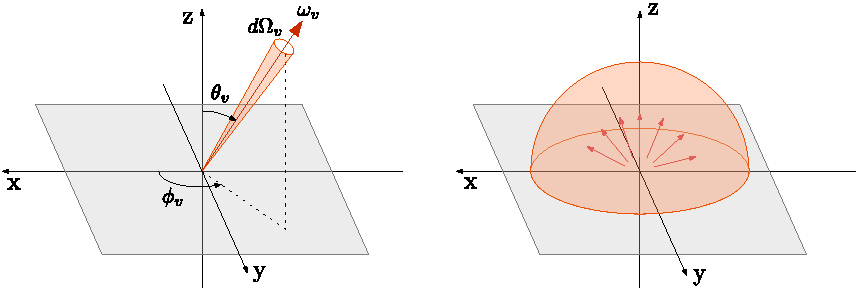
\includegraphics[width=1.0\columnwidth]{EmissivityDefinitions_Sch/EmissivityDeff.pdf}
    \caption{Schematic representation of emissivities definitions. Left: Directional Emissivity. Right: Directional emissivity.}
    \label{fig:MaxWavelenght}
\end{figure}

Unless specified otherwise, in this document, when talking about the material emissivity, we are referring to the total hemispherical emissivity. Measuring this total hemispherical emissivity will be the focus of the following sections. 

\section{Emissivity Measurement Methods}

Many methods can be used for measuring the emissivity \parencite[][]{ref:emissmeasex}. They are commonly classified as direct or indirect methods, according to the physical principle of measurements. Direct methods are those where the power radiated from the surface is measured directly: These are the so-called calorimetric and radiometric methods. 
The indirect methods, first measure the reflectivity or transmissivity of the object of interest, assuming it is not opaque. The emissivity is then calculated based on Kirchoff's laws. 

Reference \parencite[][]{ref:directMethods}, presents a detailed description of several types of direct radiometric methods, with a great number of examples that measure the emissivity using this technique. Indirect measuring examples can be found in \parencite[][]{ref:ind1}, \parencite[][]{ref:ind2}, \parencite[][]{ref:ind3}.

In our particular case, we decided to use the calorimetric method. This method consists in carrying out an energy balance of the radiative losses of the studied sample when those are the only ones to stake. The main advantage of this method is that it doesn't need sophisticated or expensive equipment, and it can measure small sample sizes. It is a direct and absolute method, which means that it does not require a referenced standard emissivity to obtain the emissivity value. 

Some disadvantages include: A constant power must be provided to the sample to maintain the temperature. The measurement is usually performed in a steady state, and therefore it is time-consuming. It is important to eliminate energy transfers by convection, thus the sample must be placed under a vacuum (typically $10^{-5}$ bar ). The biggest cause of the uncertainty of this method is the measurement of the surface temperature. This method gives us information about the total hemispherical emissivity, no information about the radiation wavelength or directionality can be obtained. 

\section{Specifics of Calorimetric Method}

The calorimetric method is based on studying the energy balance of the sample at a certain temperature. This temperature is maintained by providing power electrically by Jule effect. In this case, the energy balance of the system can be written as:

\begin{equation}
    \left(\frac{\partial T}{\partial t}\right)_{tot} = \left(\frac{\partial T}{\partial t}\right)_{Ht} - \left(\frac{\partial T}{\partial t}\right)_{Rd} - \left(\frac{\partial T}{\partial t}\right)_{Con}
    \label{eq:EneBalance}
\end{equation}

Where the Rd and Cd terms are the radiative and conduction cooling effects, introduced in chapter \ref{ch:ThermoMeasur}. In this case the heating can be expressed as: 

\begin{equation}
    \left(\frac{\partial T}{\partial t}\right)_{Ht} = \frac{I^2 R(T)}{C_p(T)\rho_v V}
\end{equation}

Here, I refer to the current applied to the wire sample and R is the resistance of that wire at a temperature T. $C_p$, $\rho_v$ and $V$ are the specific heat, the density and the volume of the wire. 

At the steady state, the temperature of the system remains constant ($\partial T/ \partial t = 0$). In this case, equation \ref{eq:EneBalance} becomes a second-order Boundary Value Problem (BVP): 

\begin{equation}
    \frac{I^2 R(T)}{C_p(T)\rho_v V} =  \frac{S \sigma_{SB} \epsilon(T) \left( T^4 - T_{0}^{4}\right)}{C_p (T) \rho_v V} + \alpha(T)\left(\frac{\partial^2T}{\partial x^2}\right)
    \label{eq:ExplicitEneBalance}
\end{equation}

Here the temperature depends only on the wire position T(x). With Dirichlet boundary conditions: 

\begin{equation}
    \begin{cases} T(0) = T_{left} \\ T(L) = T_{right} \end{cases}
\end{equation}

If one is able to properly measure the equilibrium temperature of the wire for a  given intensity, and we assume that the other material properties are known accurately, the only unknown term in equation \ref{eq:ExplicitEneBalance} is the value of the emissivity $\epsilon$(T). 

\section{Temperature Measurement}
\label{sec:EmissTempMeas}

The electrical resistance of a wire at a temperature T can be calculated as: 

\begin{equation}
    R(T) = \frac{\rho_{\Omega}(T) L(T)}{S_f}
    \label{eq:ResWithT}
\end{equation}

Where $S_f$ is the cross-section of the wire, considered to be constant over the wire length and temperature. $\rho_{\Omega}(T)$ is the resistivity of the material and L(T) is the length of the sample, both of them temperature-dependent magnitudes. The length of the sample L(T) can also change with temperature. As a first approximation, a linear model can be used: 

\begin{equation}
    \Delta L = \alpha_l \left(T - T_0 \right) \cdot L_0
\end{equation}

Where $\alpha_l$ is the coefficient of thermal expansion. It is difficult to give a mathematical description of the variation of the resistivity with temperature, as it is very much material-dependent.

Tabulated values of the electrical resistivity for different materials are well known and can be found in the literature. Usually they are expressed as the ratio between R(T) or $\rho_{\Omega}(T)$ and the resistance or resistivity at room temperature ($R_{0} , \rho_{\Omega 0}$ ) \parencite[][]{ref:HandbookCh}. Figure \ref{fig:RR0TungstenLit} shows, as an example, the resistivity of tungsten as a function of the temperature. 

\begin{figure}[h]
    \centering
    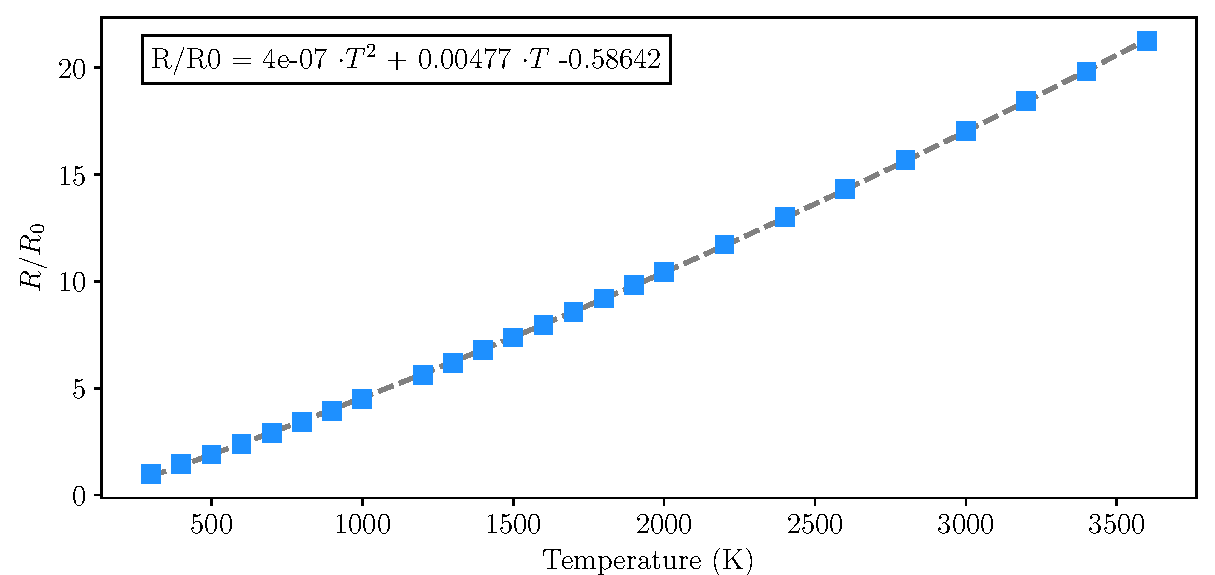
\includegraphics[width=0.85\columnwidth]{Figure_LiteratureResTemp/RR0Tungsten.pdf}
    \caption{Evolution of the R(T)/R(T0) as a function of the temperature for a tungsten wire.}
    \label{fig:RR0TungstenLit}
\end{figure}

To calculate the temperature of the average temperature of the wire material, the ratio $R/R_{0}$ was calculated experimentally for a range of applied intensities.  This was then compared to the values found in literature, that relate this ratio to temperature. In this way, a relationship between average temperature and intensity can be calculated. 

\section{Numerical Calculation of the Emissivity}
\label{sec:EmissCalc}

Equation \ref{eq:ExplicitEneBalance} can be solved numerically. As seen in chapter \ref{ch:TempModeling}, the derivatives can be approximated using the corresponding differentiation matrices associated with a set of discrete nodes. In this case, it is a little simpler as we are dealing with an ordinary differential equation, not a PDE. For this study, a central difference (CD2) was used to approximate the spatial second derivative. That is: 

\begin{equation}
    \left. \frac{d^2 T}{dx^2}\right|_{x_i} = \frac{T_{i+1}-2T_i + T_{i-1}}{2\delta_x^2} + \mathcal{O}(\delta_x^2)
\end{equation}

Rewriting this system in a matrix form yields: 

\begin{equation}
    \begin{bmatrix}
   1 &  0 & 0 & 0 & 0 & 0\\
   1 & -2 & 1 & 0 & 0 & 0\\
   0 & 1 & -2 & 1 & 0 & 0\\
   0 & 0 & \ddots & \ddots & \ddots & 0 \\
   0 & 0 & 0 & 1 & -2 & 1 \\
   0 & 0 & 0 & 0 & 0 & 1
   \end{bmatrix}
   \begin{bmatrix}
       T_0 \\ T1 \\ T2 \\ \vdots \\ T_N \\ T_{N+1}
   \end{bmatrix}
    = 
\begin{bmatrix}
   f_0 \\ f1 \\ f2 \\ \vdots \\ f_N \\ f_{N+1}
\end{bmatrix}
\end{equation}

Where $T_i$ are the unknowns of the BVP. $f_0 = T_{left}$ and $f_N = T_{right}$. While the rest can be written as:

\begin{equation}
    f_i = \delta^2_x \cdot \left( A + B T^4_i \right)
\end{equation}

With $A = -\frac{1}{\alpha}\left(I^2 R + S\epsilon \sigma_{SB}T_0^4\right)$ and $B = \frac{1}{\alpha}S \sigma_{SB}\epsilon$. Due to the $T_i^4$ term, this is a nonlinear system of equations. For solving this system of equations Newton's method for nonlinear systems was used \parencite[][]{ref:AlvaroBook}. In this case, tolerance of $10^{-8}$ was considered. Reached this point, the reader might be asking themselves, wasn't we trying to calculate the emissivity? wasn't the temperature known? 

From how the experiment was performed, we could measure the average temperature of the wire ($T_{meas}$). This temperature is not constant along the wire length, for that reason, to compare the simulated values of the temperature $T_{i}$ to the measured value ($T_{meas}$) we have to first calculate the mean temperature of our thermal profile. 

\begin{equation}
    T_{sim} = \frac{1}{L}\int_{0}^{L} T(x) dx
\end{equation}

To calculate the emissivity of the material, an iterative method was used. The steps to find the solution are the following: 

\begin{enumerate}
    \item An initial guess of the emissivity is provided ($\epsilon_i^0$, where the super-index indicates the iteration number).
    \item With this value of the emissivity, the BVP is solved and then the average temperature along the wire is calculated ($T^{n}_{sim}$). 
    \item The calculated value of the temperature is compared to the experimentally measured one: 
    \begin{equation}
        e^{n} = T^{n}_{sim} - T_{meas}
    \end{equation}
    If the simulated temperature is higher than the measured one, it means that the cooling should be stronger, that is, the value of the emissivity should be higher. Conversely, if the simulated temperature is smaller than the measured one, the value of the emissivity should be reduced. 

    \item The value of the emissivity is updated as follows: 
        \begin{equation}
               \epsilon^{n+1}_j = \begin{cases}  (\epsilon^n_j + 1)/2, & \mbox{if } e^n > 0\\ (\epsilon^n_j)/2, & \mbox{if } e^n < 0 \end{cases}
         \end{equation}
    \item This process is repeated until convergence.
\end{enumerate}

If the initial guess of the emissivity is between 0 and 1, the iterative process always keeps it in this range. The convergence condition is met once $\left| \epsilon^{n} - \epsilon^{n+1}\right| < 10^{-3}$. If converge condition is never met, iteration stops when the number of iteration reaches $it_{max} = 50$. A detailed study of the residuals was also performed when the convergence condition was met.  

\section{Experimental Set Up}

The experimental setup was designed and put together with the huge assistance of Miguel Martin \footnote{miguel.martin.nieto@cern.ch}, who implemented from scratch the electronics used for this experiment. The setup consisted of: Power Supply, Acquisition system, Vacuum system and Sample. Picture \ref{fig:ExperimentalSetUp} shows a picture of full experimental set up. The total cost of the experiment was under 300 CHF as most of the equipment was already available. 

\begin{figure}[h]
    \centering
    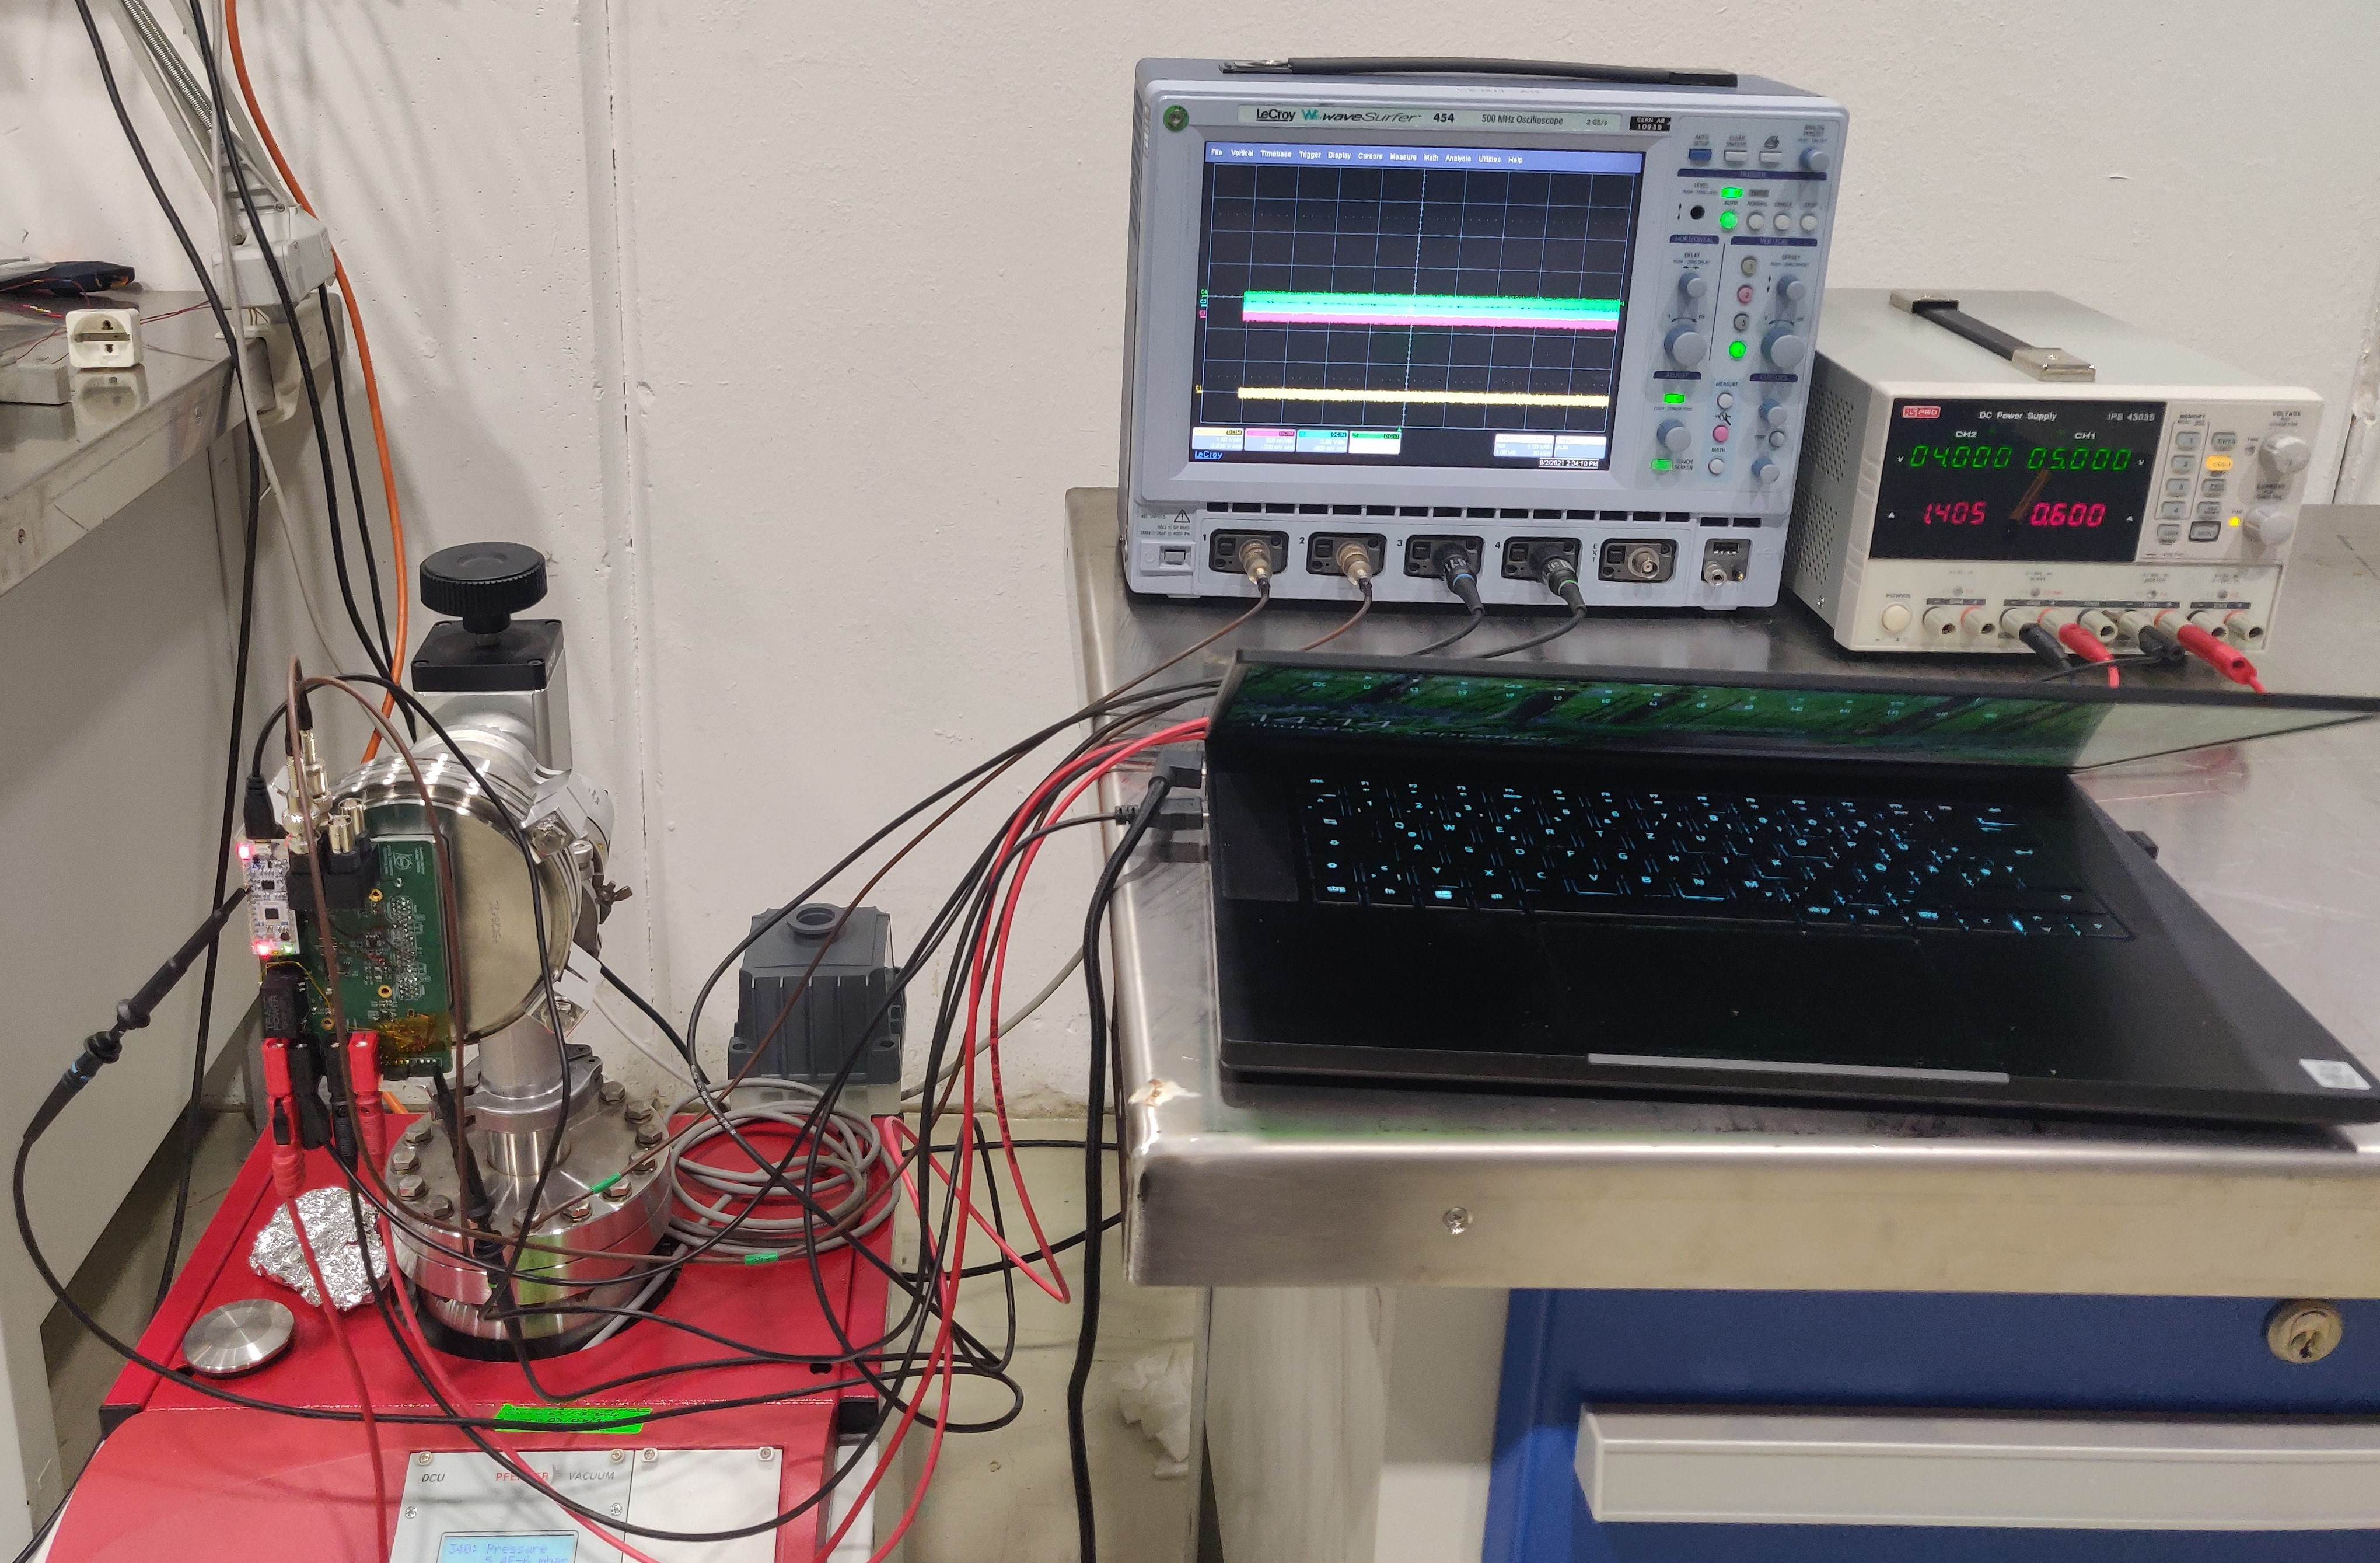
\includegraphics[width=0.65\columnwidth]{ExperimentalSetUp/ExperimentalSetUp.jpg}
    \caption{Picture of the experimental setup for emissivity measurements.}
    \label{fig:ExperimentalSetUp}
\end{figure}

The system was powered by a lab power supply. On-board DC-DC converters and linear regulators in the acquisition system adapted the input voltage to the levels necessary to power the various analog parts of the circuit. An oscilloscope was sometimes used to monitor intermediate signals in the acquisition system and guarantee accurate measurement results. The measurements were automatized and controlled via a python code. The measured data was also automatically stored and an on-the-fly analysis could be performed to cross-check the quality of the results. 

A HiCube300 Eco, was used to create the necessary vacuum ($10^{-5}$ bar) in the vacuum chamber. This pump includes a turbopump and a backing pump for achieving high vacuum applications ($10^{-7}$ mbar). A vacuum gauge was available to continuously monitor the vacuum levels. 

\subsection{Adquisition system}

The acquisition system consists of an assembly of two circuit boards: the measuring board and the acquisition board. A schematic representation of the electronic setup is shown in figure \ref{fig:SchemaElectronics}. 

\begin{figure}[h]
    \centering
    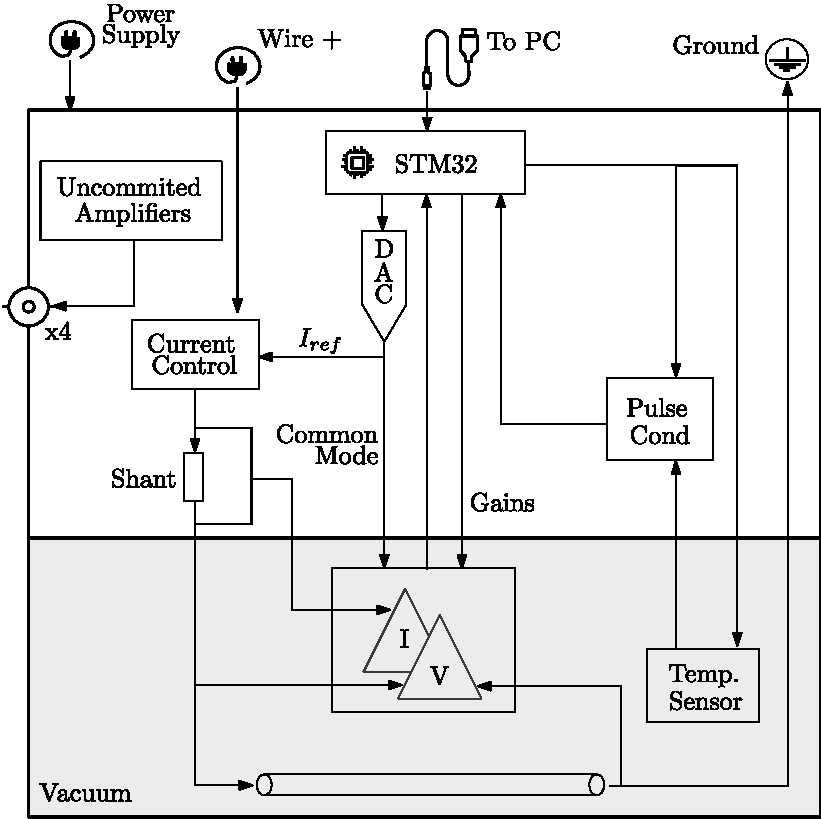
\includegraphics[width=0.65\columnwidth]{ElectronicSchema/ElectronicSchema.pdf}
    \caption{Schematic representation of the electronics set up. }
    \label{fig:SchemaElectronics}
\end{figure}

The measuring board had two main objectives: holding the wire with both ends and measuring the current and voltage drop in the wire. Figure \ref{fig:MeasuringBoard} shows a 3D design of this board. The wire was fixed on two of the turrets at a set distance. The redundancy on the turret number allowed for measuring wires of different lengths. This board was placed inside the vacuum chamber, its size and design had to be added to its shape. 

\begin{figure}[h]
    \centering
    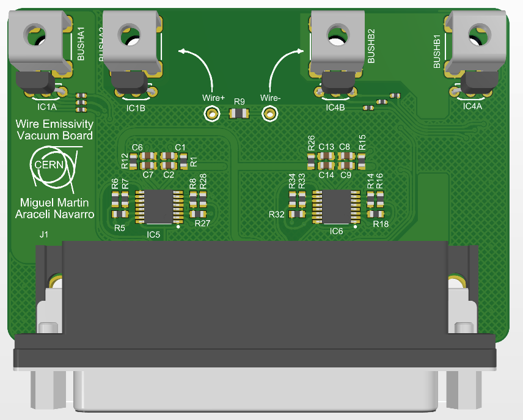
\includegraphics[width=0.5\columnwidth]{3DBoardDesigns/MeasuringBoard.png}
    \caption{3D design of the Measuring board.}
    \label{fig:MeasuringBoard}
\end{figure}

The intensity is measured using a shunt resistor, which was placed in the acquisition board outside of the vacuum to facilitate heat dissipation. The voltage drop in the wire is measured directly at the mounting points, ensuring that only the voltage drop developed in the wire is taken into account. The vacuum feed-through connector is installed on the board, to transmit the signals across the vacuum barrier. The range of voltage (0 - 6V) and intensity (0 - 2 A) to be measured was quite broad. To overcome the limited range of the ADCs, different gains are available on the amplifiers. The temperature at the extremes of the wire ($T_{left}, T_{right}$) is measured by means of two temperature sensors mounted on the turrets. 

The acquisition board captures and digitalizes the measured signals, regulates the current flowing into the wire and configures the measurement board for gain and common-mode offset. Figure \ref{fig:AdquisitionBoard} shows a 3D design of this board. 

The measured current and voltage signals are digitalized by the dual differential ADCs built into the microcontroller. A pulse conditioning block adapts the signal from the temperature sensor to the logic levels used by the microcontroller. The current, voltage and temperature signals are sent to a computer at a settable interval (minimum $100 \mu s$) via a 1-Mbps USB serial connection. Four uncommitted amplifiers with BNC connectors are available to cross-check various signals with external equipment. 

\begin{figure}[h]
    \centering
    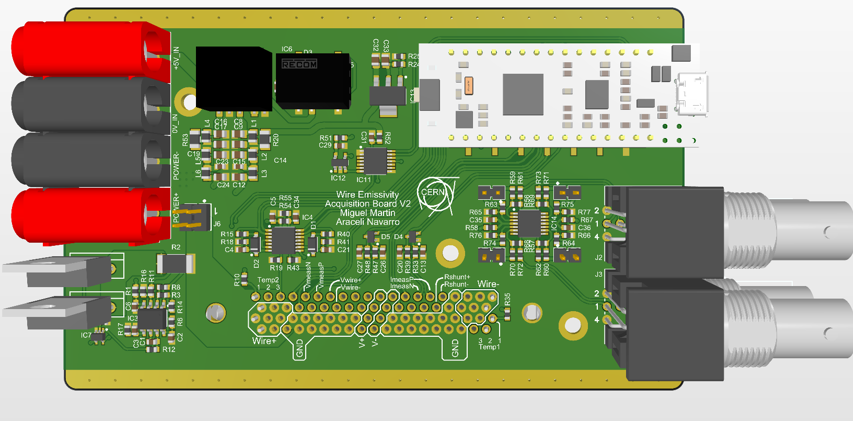
\includegraphics[width=0.8\columnwidth]{3DBoardDesigns/AdquisitionBoard.png}
    \caption{3D design of the acquisition board.}
    \label{fig:AdquisitionBoard}
\end{figure}

\section{Adquisition System Calibration}

Before proceeding with the measurements, the acquisition boards had to be calibrated. That means one has to make sure that the voltages and currents registered by the data acquisition system are the same as the ones truly going through the wire. To cover the full range of intensity and voltage to be measured different gains were available on the amplifiers. These gains are summarized in table \ref{tab:AvGains}. A calibration curve had to be calculated for each amplification option. 

\begin{table}[h]
    \centering
    \begin{tabular}{ccc}
    \hline
    Name & Amplification & Magnitude \\ \hline
    GV0  & Voltage       & x 0.5     \\
    GV1  & Voltage       & x 1       \\
    GV2  & Voltage       & x 2       \\
    GI0  & Intensity     & x 1       \\
    GI1  & Intensity     & x 2       \\ \hline
    \end{tabular}
    \caption{Summary of available voltage and amplification options. }
    \label{tab:AvGains}
\end{table}

The calibration was performed outside of vacuum, by comparing the voltage and the current registered by the acquisition system after the digitalization to an independent measurement taken at the extremities of the wire, before any amplification was performed. This independent measurement was performed using a Keithley 2001 multi-meter for voltage measurements and a FLUKe 289 true RMS multi-meter for the intensity measurements. Figure \ref{fig:CalibrationCurves} shows the calibration curves of the acquisition system as a function of the current given to the system. All of the curves show clear linearity, demonstrating the electronics behave as expected. We will refer to the real current and voltage going through the wires as $I_{real}$ and $V_{real}$, while the current and the voltage provided are $I_{adc}$ and $V_{adc}$. The linear fits for the different curves are: 

\begin{equation}
    \textcolor{gray}{I0:} \qquad I_{real} = 0.969 \cdot I_{adc} + 0.0045
\end{equation}
\begin{equation}
    \textcolor{orange}{I1:} \qquad I_{real} = 0.547 \cdot I_{adc} + 0.0027
\end{equation}
\begin{equation}
    {\color{CornflowerBlue}{V0:} }\qquad V_{real} = 2.313 \cdot V_{adc} - 0.0293
\end{equation}
\begin{equation}
    \textcolor{BrickRed}{V1:} \qquad V_{real} = 1.071 \cdot V_{adc} - 0.0175
\end{equation}
\begin{equation}
    \textcolor{ForestGreen}{V2:} \qquad V_{real} = 0.525 \cdot V_{adc} - 0.0071
\end{equation}
    
Note that for convenience these equations are given as the inverse fitted curves in figure \ref{fig:CalibrationCurves}. The saturated points were not used for the calculation of these curves. The values of the voltage and the intensity used in the following sections are the real ones, calculated using these calibration curves.

\begin{figure}[h]
    \centering
    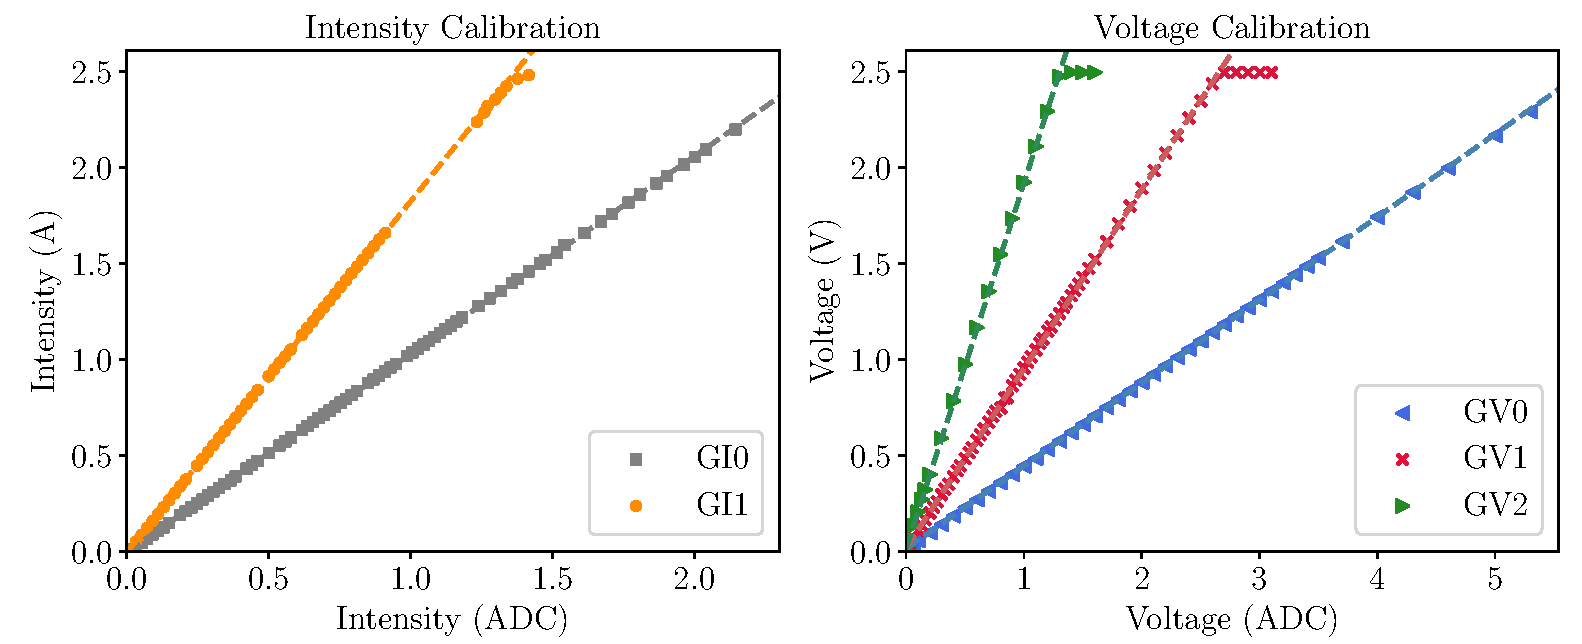
\includegraphics[width=1.0\columnwidth]{Figure_CalibrationCurves/CalCurve.pdf}
    \caption{Calibration curves for the different amplification ranges. Left: Intensity Calibration. Right: Voltage Calibration. The explicit expression of the fitted curves (dashed lines) is provided in the text. }
    \label{fig:CalibrationCurves}
\end{figure}

\section{Experimental Results}

For this analysis, Tungsten wires of two different diameters ($10 \mu m$ and $40 \mu m$) were measured. Both, with and without gold coating. For each type of wire, four samples were measured in order to compile some statistics. 

\subsection{Steady State Determination}

In figure \ref{fig:RawMeasurements} the raw data (before calibration) for the intensity, voltage and resistance is presented as a function of time. The applied intensity for the three figures on the left was 50 (mA) whereas for the three figures on the right was 190 (mA). The measured intensity remains constant along the measurement time as it is externally provided to the wire. The time it takes the voltage to stabilize reflects the change in the resistance of the wire for the applied intensity. The resistance was calculated from the previous two measurements using Ohm's law. 

\begin{figure}[h]
    \centering
    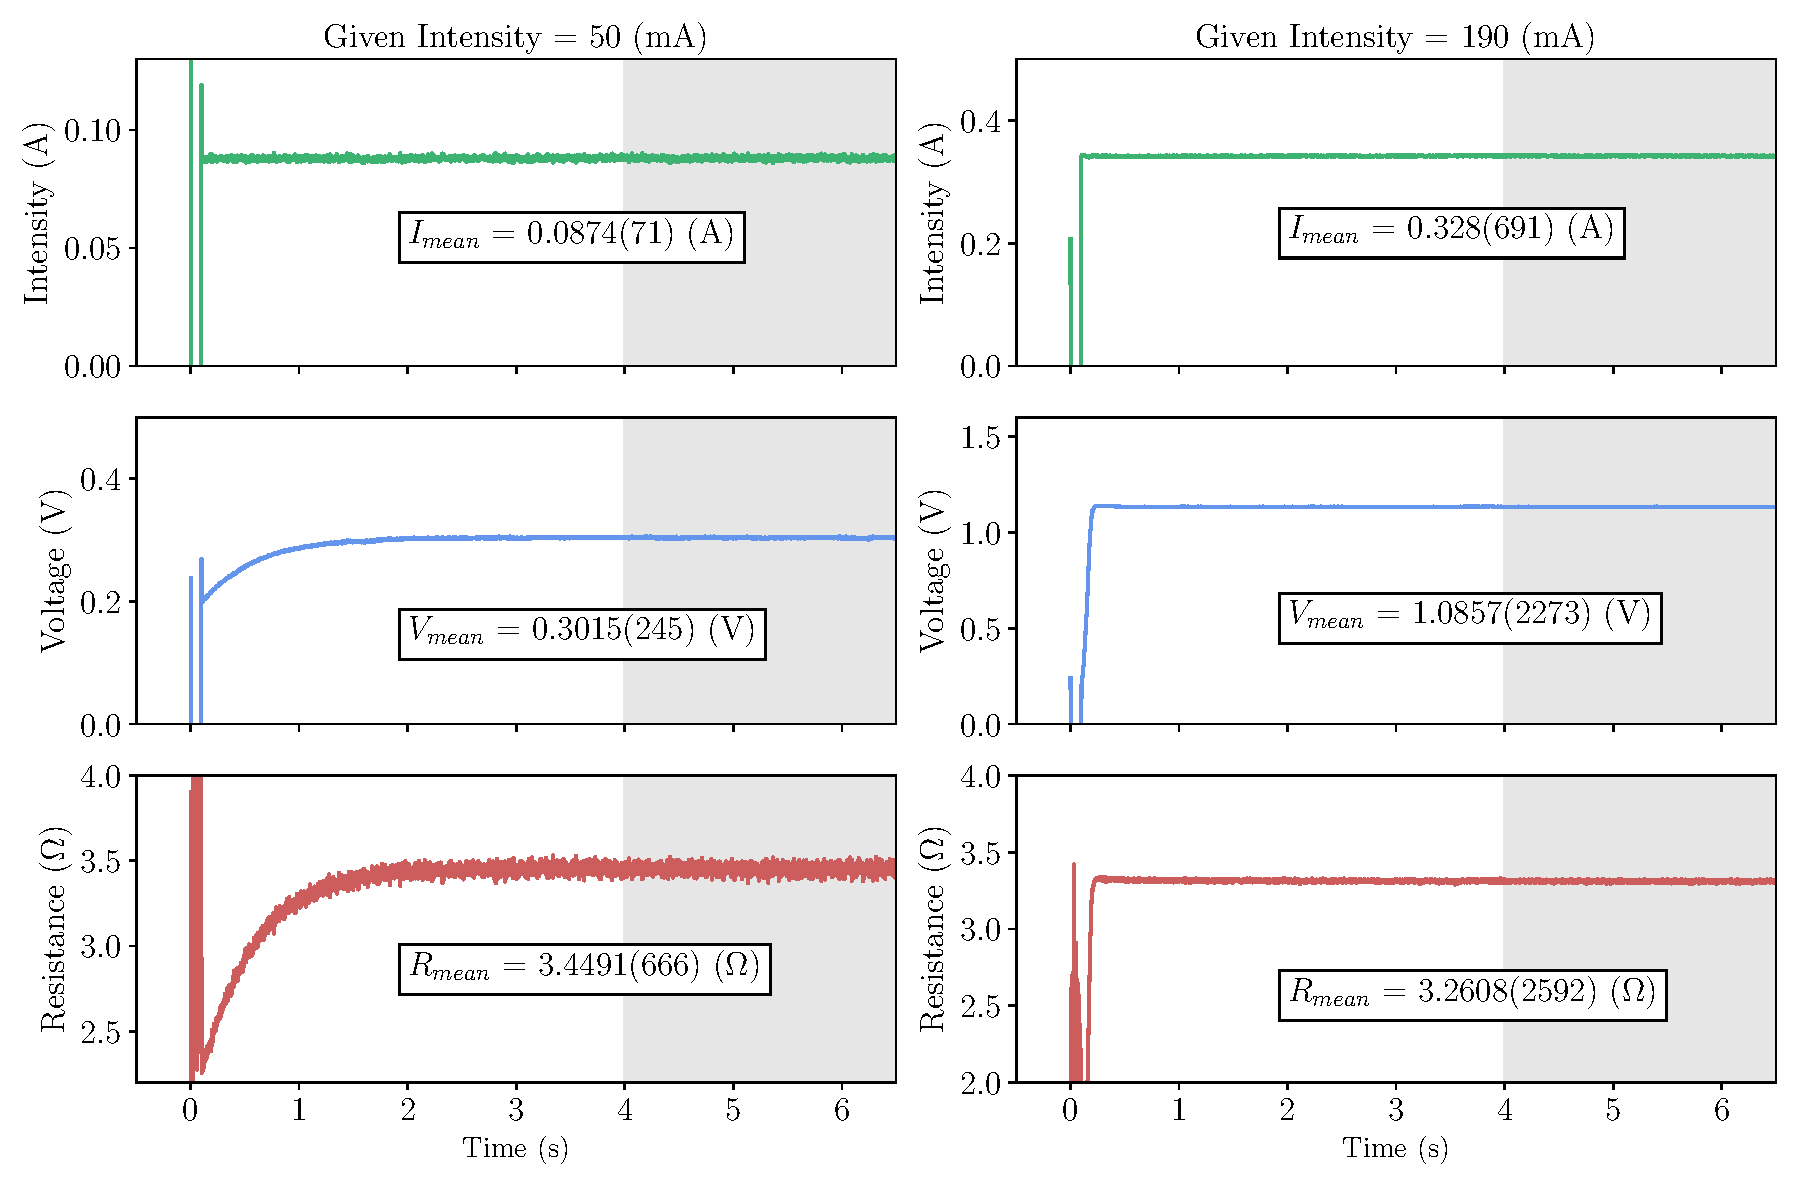
\includegraphics[width=1.0\columnwidth]{Figure_TransientExample1/TransientExample.pdf}
    \caption{Raw data measurements (before calibration) for a 40 $\mu m$ gold-coated tungsten wire. Intensity, voltage and resistance as a function of time for an applied current of 50 mA (left) and 190 mA (right). The mean values of the different quantities were calculated in the gray area. }
    \label{fig:RawMeasurements}
\end{figure}

We consider the steady state has been reached when the values of the voltage and the resistance remain stable along time ($dV/dt = dR/dt = 0 $).  This starting point is calculated by evaluating when the derivative of the measurements is smaller than $10^{-2}$. The derivative was numerically calculated on a window of the measured data to overcome the measurement noise. 

\begin{figure}[h!]
    \centering
    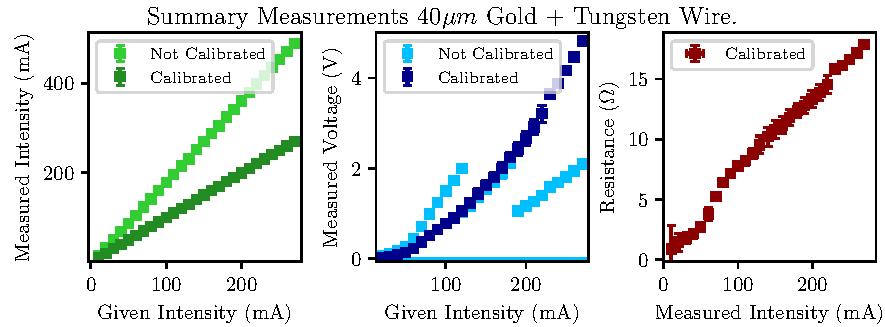
\includegraphics[width=1.0\columnwidth]{Figure_MeasuredValues_IVR/40AuW.pdf}
    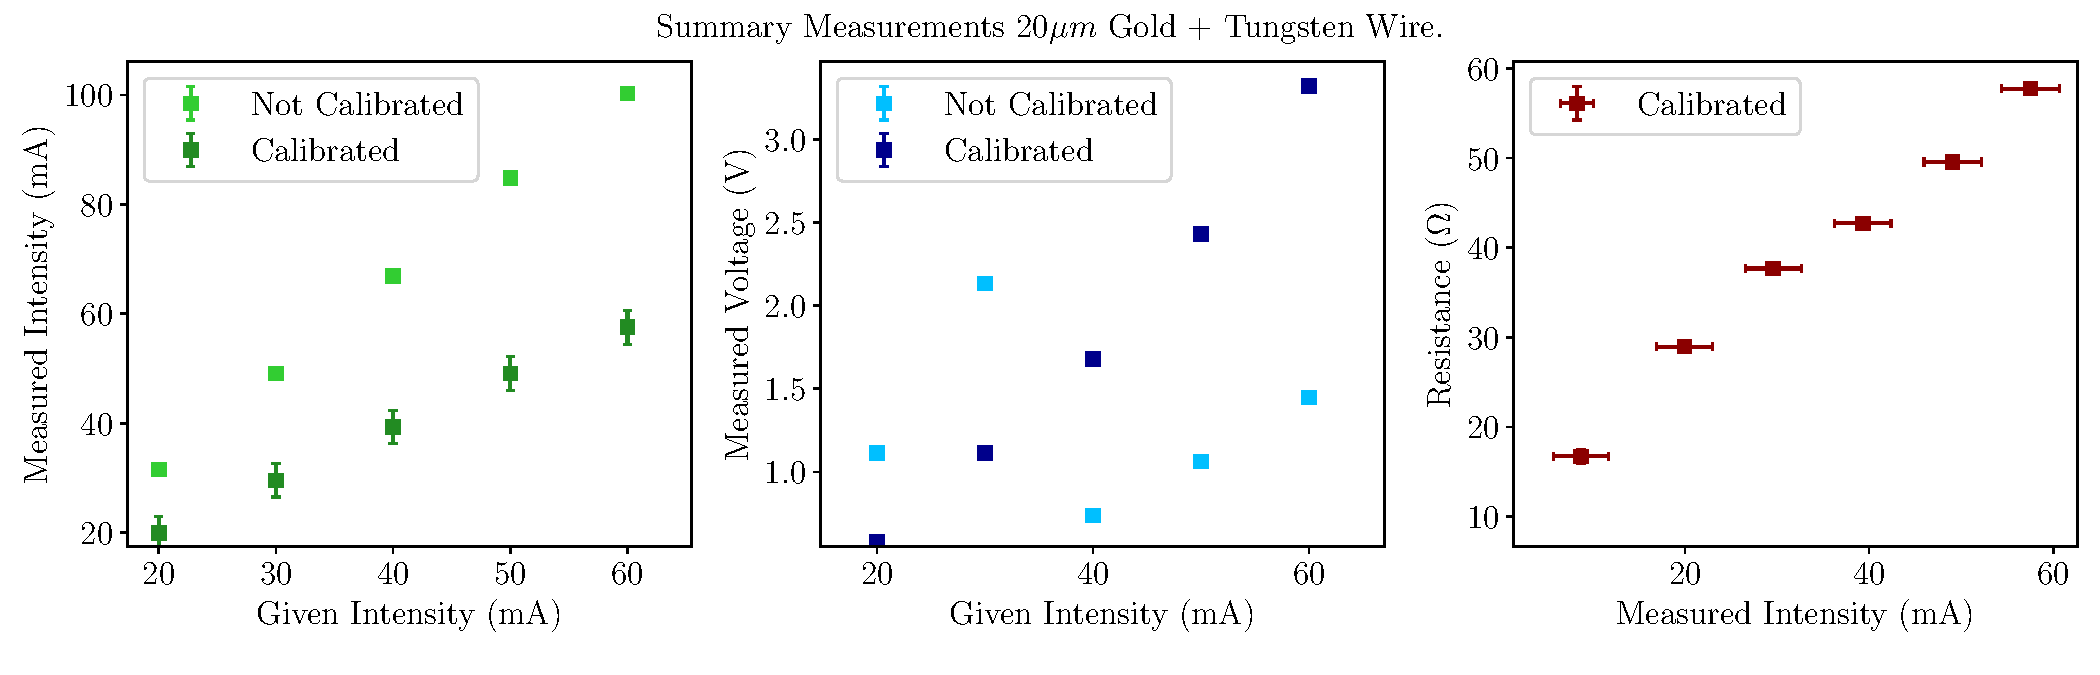
\includegraphics[width=1.0\columnwidth]{Figure_MeasuredValues_IVR/20AuW.pdf}
    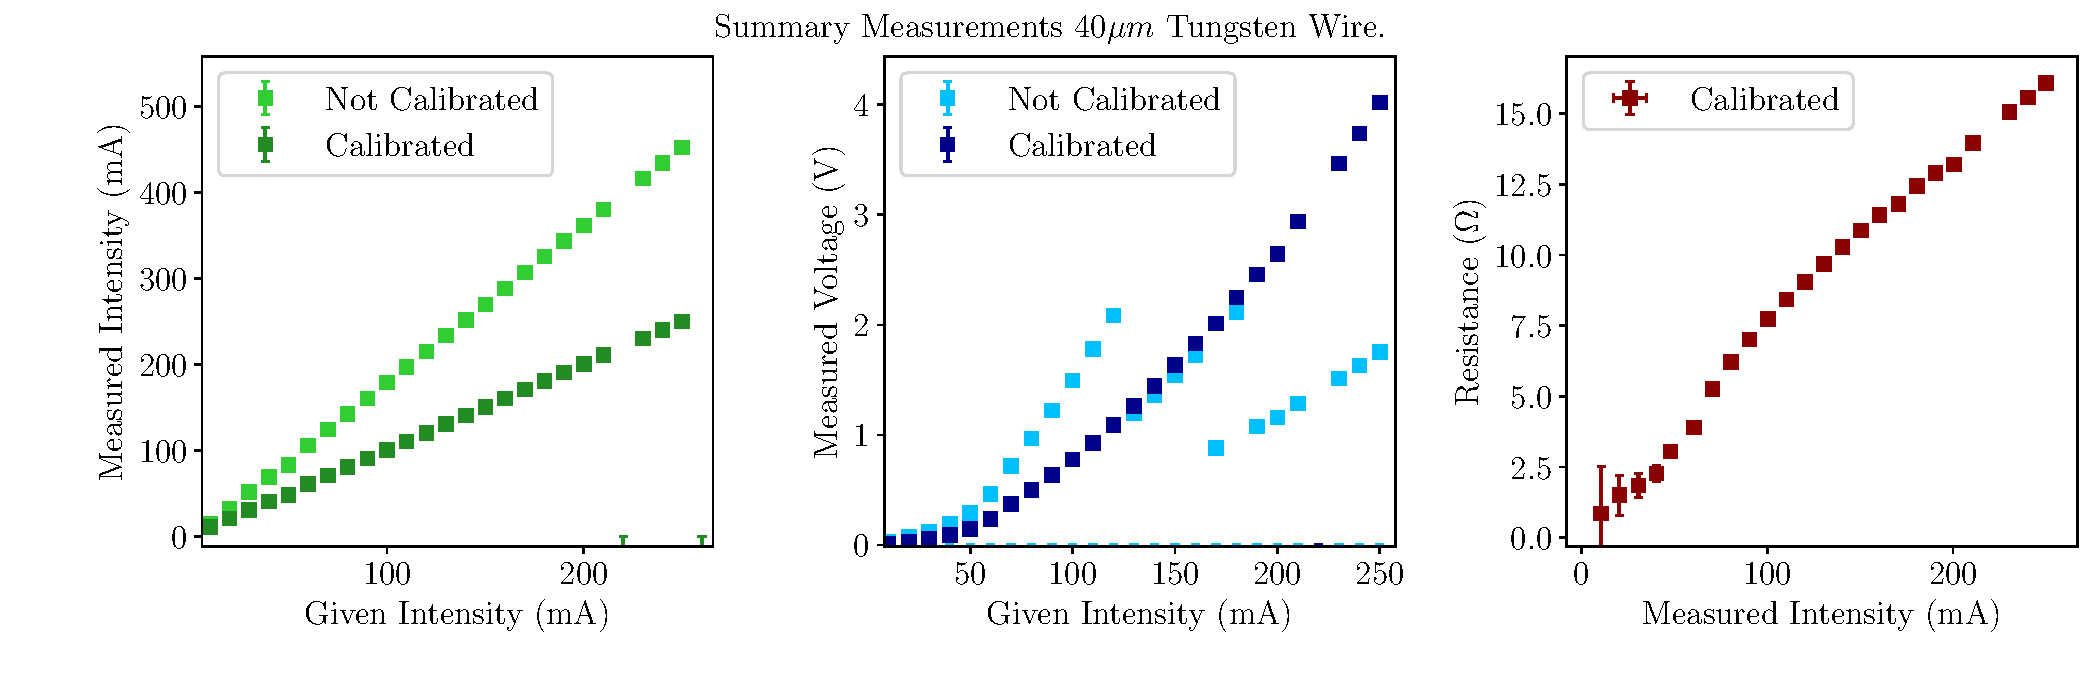
\includegraphics[width=1.0\columnwidth]{Figure_MeasuredValues_IVR/40W.pdf}
    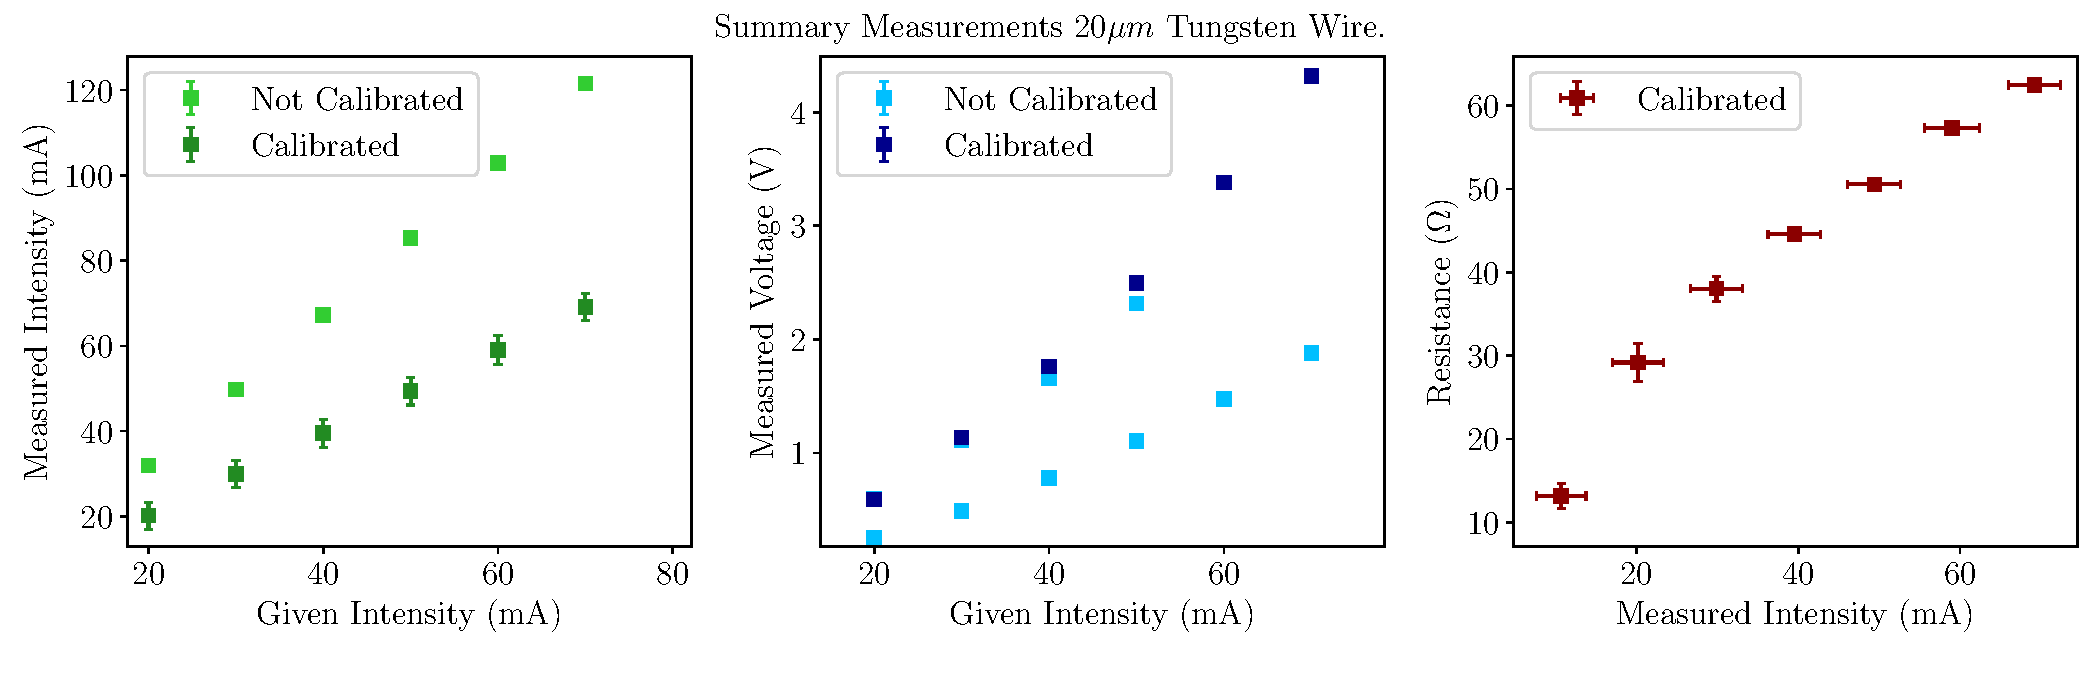
\includegraphics[width=1.0\columnwidth]{Figure_MeasuredValues_IVR/20W.pdf}
    \caption{Summary of the measured intensity (left), voltage (center) and resistance(right), on the steady state, for the different samples as a function of the applied intensity. }
    \label{fig:SummarySteadyState}
\end{figure}

For each applied intensity the steady-state values were calculated and conveniently stored. Figure \ref{fig:SummarySteadyState} shows a summary of the intensity, voltage and resistance measured (on the steady state) for the different wires. The error bars in these plots show how much the measurements varied between samples of the same wire type. In these figures, we can observe how different gains needed to be used to cover all the voltage ranges. The $20 \mu m$ wires show a resistance $\sim 4$ times higher than the resistance measured for the $40 \mu m$ wires, which is in agreement with equation \ref{eq:ResWithT} assuming a very similar resistivity as the material was the same. The voltage increase for the smaller wires was also much larger than for the bigger wires, consistent with this resistance difference. 

\subsection{Intensity Temperature Curves}

The average temperature for each applied intensity was determined following the procedure explained in section \ref{sec:EmissTempMeas}. First, the value of $R_0$ (Resistance at ambient temperature) was calculated. Measuring $R_0$ implies measuring the resistance with no current applied to the wire, which could not be done in reality. To calculate this, the measurement points (R,I) at very low current were extrapolated to zero using a parabolic model: $R(I) = R_{0} + A\cdot I^2$. Figure \ref{fig:R0Calc} shows how the value of $R_0$ was calculated for the gold-coated tungsten wire. 

\begin{figure}[h!]
    \centering
    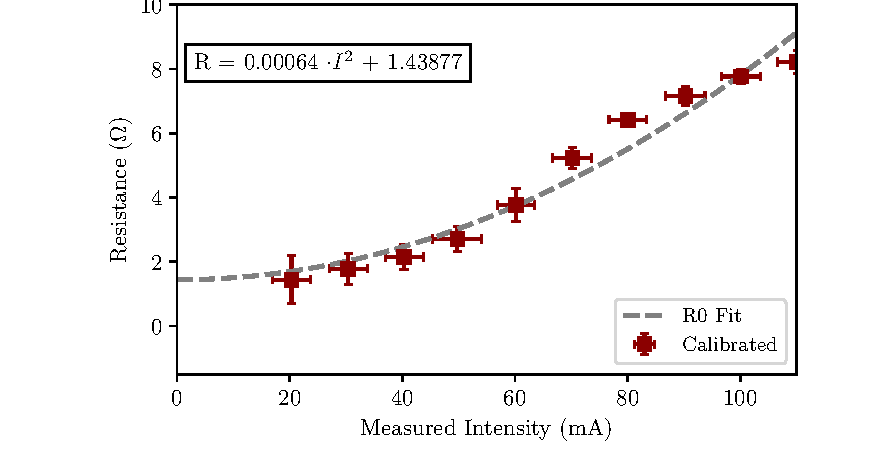
\includegraphics[width=0.8\columnwidth]{Figure_CalculateR0/CalcR0.pdf}
    \caption{Calculation of $R_0$ for a $40 \mu m$ Tungsten wire. Only the first 8 points were considered for the fitting. }
    \label{fig:R0Calc}
\end{figure}

A summary of the calculated values of $R_0$ for the other wire types can be found in table \ref{tab:R0table}. Note that the relative error when calculating $R_0$ for the 40 $\mu m$ wires was smaller than $7\%$. However, the relative error for the 20 $\mu m$ wires bordered $60 \%$. This much bigger error in the case of smaller wires comes from the too coarse intensity scan. Unfortunately, the time restrictions prevented getting a much more accurate measurement. 

\begin{table}[h]
    \centering
    \begin{tabular}{ccc}
    \hline
    Composition          & Radius ($\mu m$) & $R_0$ ($\Omega$) \\ \hline
    \multirow{2}{*}{AuW} & 20               & 10.5(63)         \\
                         & 40               & 1.438(76)        \\
    \multirow{2}{*}{W}   & 20               & 11.1(53)         \\
                         & 40               & 1.562(58)        \\ \hline
    \end{tabular}
    \caption{Summary of $R_0$ values for the different wire types. }
    \label{tab:R0table}
\end{table}

To calculate the wire temperature as a function of the intensity we compared the values of the measured ratios $R/R_{0}$ with the ones one finds in the literature. Because the resistivity is a body effect, the resistivity that we considered was the one of Tungsten. Figure \ref{fig:MeasTempCurrent} shows a summary of the average temperatures measured as a function of the measured intensity. A range of average temperatures, ranging from room temperature to almost 2500K, was covered during the experiments. The big uncertainties when calculating $R_0$ in the case of the 20 $\mu m$ wires yielded huge uncertainties in the average temperature calculation. Due to these big uncertainties, we considered these results unable to be used for accurately calculating the emissivity of the material.  

\begin{figure}[h]
    \centering
    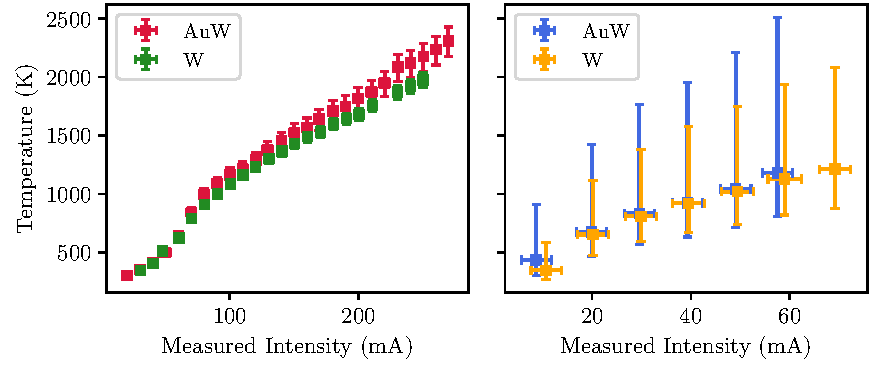
\includegraphics[width=1.0\columnwidth]{Figure_CalculatedIntTemp/IntensityTemp.pdf}
    \caption{For the different types of wires, average temperature as a function of the intensity going through the wires.}
    \label{fig:MeasTempCurrent}
\end{figure}

\subsection{Boundary Condition Measurements}

The temperature at the extremes of the wire ($T_{left}, T_{right}$) was measured by two temperature sensors in direct contact with the turrets holding the wire. As an example of boundary thermal measurements, figure \ref{fig:ExtremeTempMeas} shows the temperature at the extremes, as a function of time, for several different applied currents. For higher applied intensities larger the temperature increase in turrets. Also, the rate at which the temperature increased and the time it took for it to stabilize was dependent on the applied current. In this figure, we can see an example of how the turrets were cooling down after a measurement (red and orange curves). In this case, the cross indicates the instant of time when intensity stopped being applied to the wire. 

\begin{figure}[h]
    \centering
    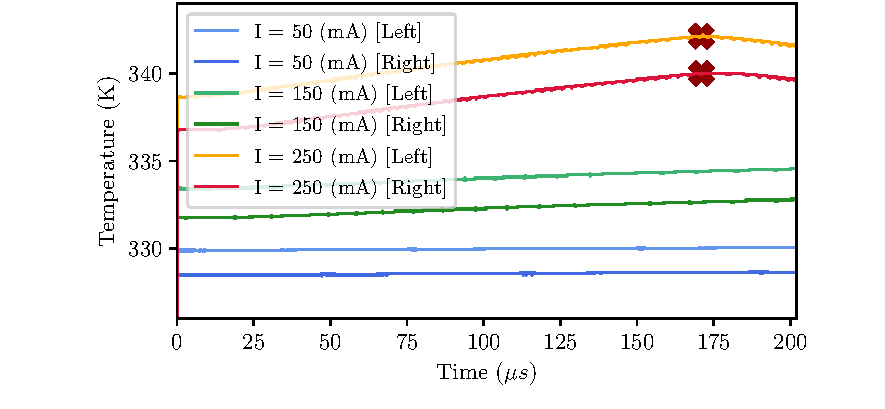
\includegraphics[width=0.8\columnwidth]{Figure_TrightTleft/TleftTright_time.pdf}
    \caption{Measurement of $T_{right}$, $T_{left}$ as a function of time for different applied currents. The red crosses indicate the point when intensity sopped is being provided to the wire.}
    \label{fig:ExtremeTempMeas}
\end{figure}

For the measurements, we also took into account the time evolution of $T_{left}$ and $T_{right}$ to calculate the starting point of the steady state. However, in some cases, the measurements were stopped before full equilibrium was achieved due to the long time it took for the boundary temperature to stabilize and the small increase rate. Figure \ref{fig:summaryTleftTright} shows the equilibrium or quasi-equilibrium values of $T_{left}$ and $T_{right}$ measured as a function of the intensity going through the wire. The boundary temperature seemed to exponentially increase with the current applied. In all the range of measurements, the temperature increase remained smaller than 350 K.

\begin{figure}[h]
    \centering
    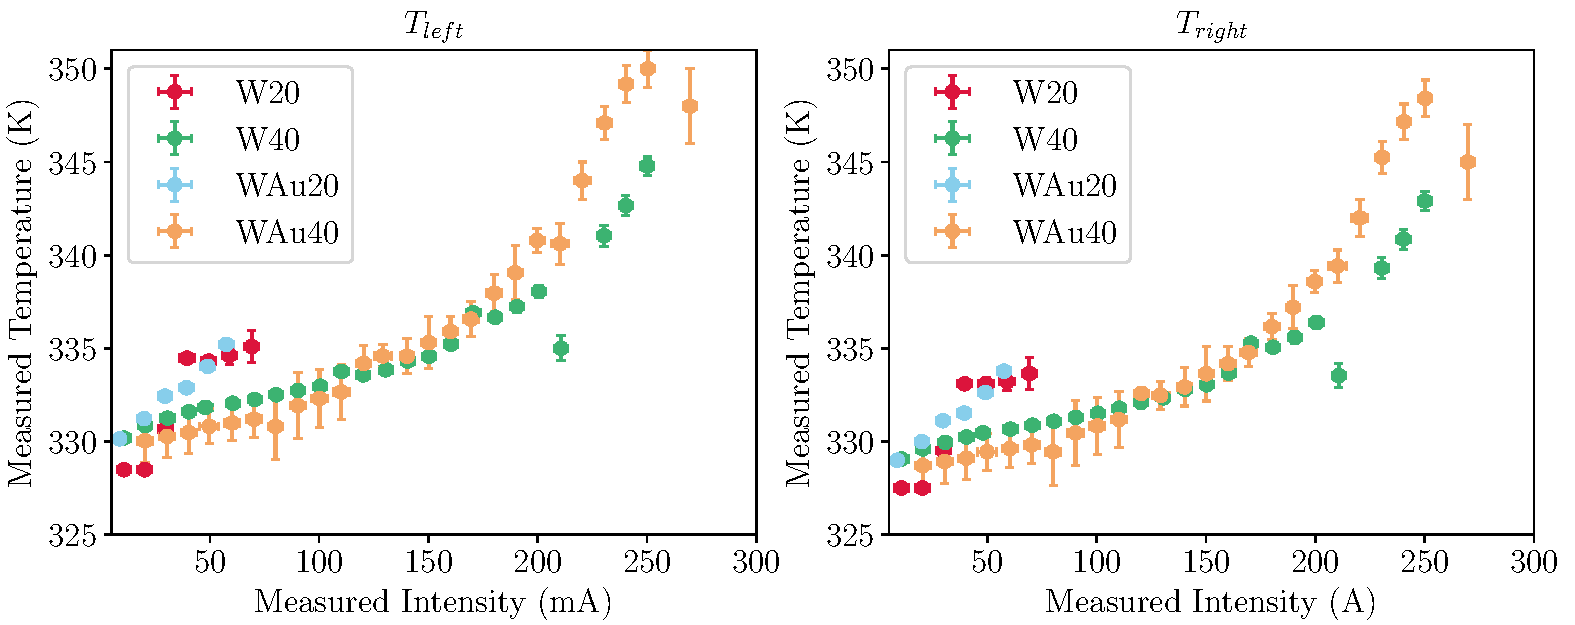
\includegraphics[width=1.0\columnwidth]{Figure_TrightTleft/TleftTright.pdf}
    \caption{Summary of boundary temperatures ($T_{left}$, $T_{right}$) measured by the thermo-couples at the extremes of the wire for different applied currents}
    \label{fig:summaryTleftTright}
\end{figure}

\subsection{Wire Emissivity}

For all the measured (Intensity, Temperature) range of points, the emissivity of the wire was calculated following the procedure indicated in section \ref{sec:EmissCalc}. As an intermediate result, figure \ref{fig:ThermalProfile} shows some examples of the equilibrium thermal profiles along the wire length. From this figure, we can see how the thermal profiles change as the applied intensity increases. At higher intensities (higher temperatures) the thermal profile is almost constant, and one could even simplify the problem by considering there is no conduction cooling in the energy balance \parencite[]{ref:tungstenemissi}. This approximation highly simplifies the numerical study of the problem however for lower average temperatures this is no longer a valid approach. 

\begin{figure}[h!]
    \centering
    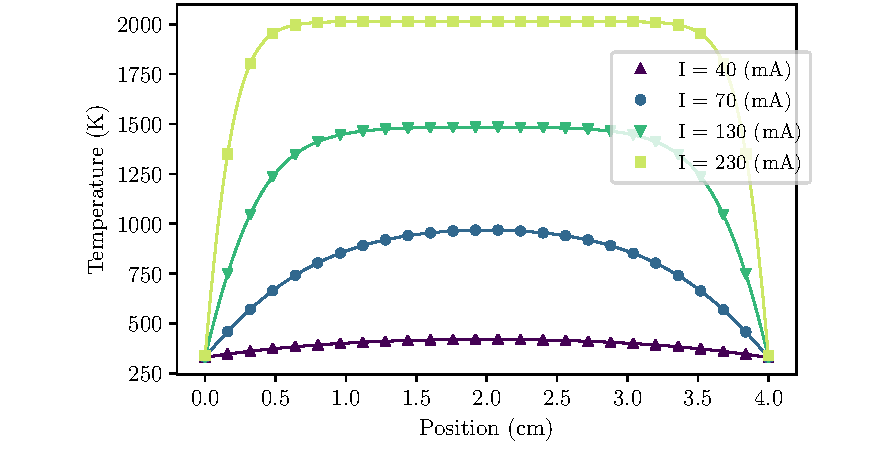
\includegraphics[width=0.75\columnwidth]{TempProf/TempProfPlot.pdf}
    \caption{Steady state temperature profile calculated for different intensities.}
    \label{fig:ThermalProfile}
\end{figure}

The emissivity of the material was calculated numerically for all the measured intensity ranges. For the pure tungsten wires, the numerical method did not converge for temperatures smaller than 500K. Similarly, for the gold-coated wires, the method only converged for average temperatures larger than 750K. The emissivity for 20 $\mu m$ wires could not be calculated due to the high uncertainties in the temperature measurements. Figure \ref{fig:EmissivityCalculations} shows the computed values for the emissivity of the 40 $\mu m$ tungsten wires. 

For both, gold-coated tungsten wires and pure tungsten wires, the emissivity increased as the temperature increased. The average emissivity of pure tungsten wires was systematically larger than the emissivity measured for the gold-coated wires. Going back to figure \ref{fig:EmissUnc}, one can observe how the measured emissivity of the gold-coated wires matches very well the previously reported values of the wire emissivity. For tungsten, both the slope and the measured values agree with some of the published references, particularly those reporting values of poorer electromagnetic radiators. 

\begin{figure}[h]
    \centering
    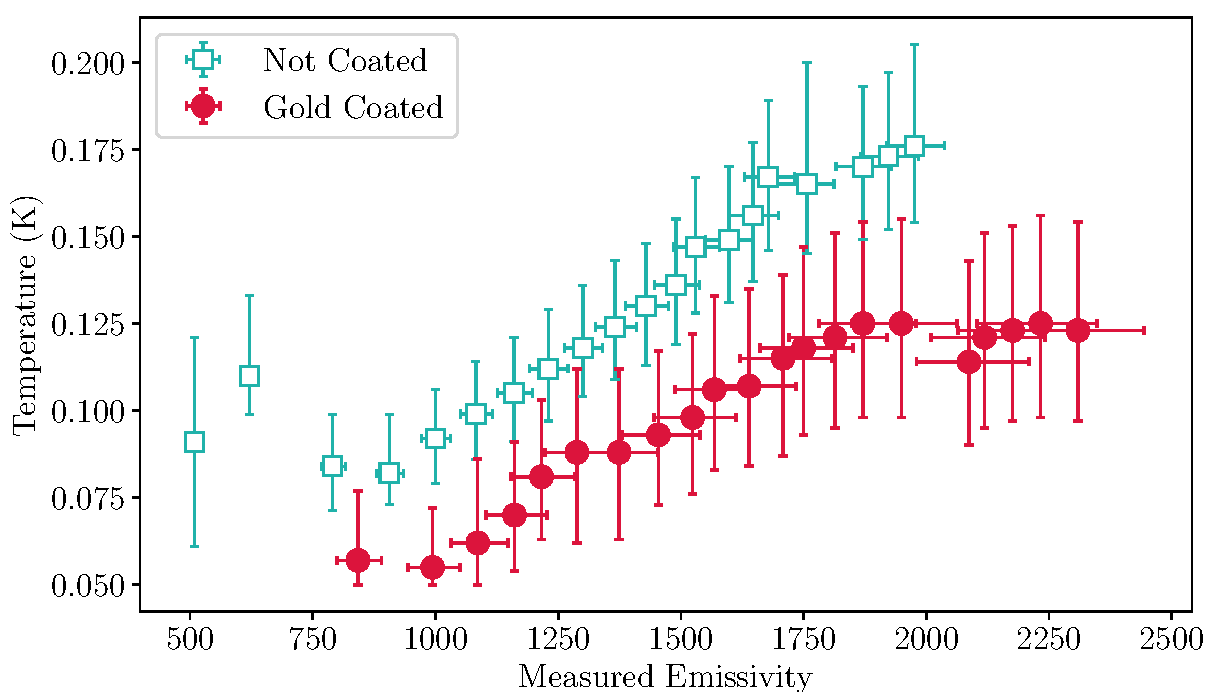
\includegraphics[width=0.8\columnwidth]{EmissivitySummary/EmissivitySummaryPlot.pdf}
    \caption{Measured emissivity for 40 $\mu m$ tungsten wires as a function of the temperature.}
    \label{fig:EmissivityCalculations}
\end{figure}

\subsection{Convection Effects}

Convection cooling is the mechanism where heat is transferred from the hot device by the flow of the fluid surrounding the object. If the exeriment had been done in air, this convective term should have been considered. A very simple way of modeling could be: 

\begin{equation}
    \left(\frac{\partial T}{\partial t}\right)_{Cnv} = \frac{hA\left(T - T_{f} \right)^{b}}{V\cdot C_{p}(T)\cdot \rho_v(T)}
\end{equation}

Where A is the area of the object, h is the heat transfer temperature, $T_f$ is the fluid temperature and b is the scaling exponent \parencite[][]{ref:Convection}. The heat transfer coefficient is highly dependent upon the physical properties of the fluid and the experimetal conditions. The values for h have been measured at tabulated and can be found in literature. However, the uncertainties this coefficient introduce great uncertainties in our energy valance equation, dificulting the calculation of the wire emissivity. 

\begin{figure}[h]
    \centering
    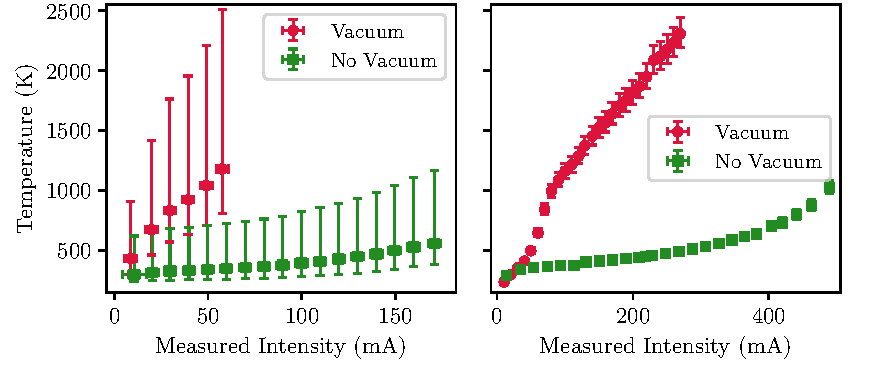
\includegraphics[width=1.0\columnwidth]{Figure_ConvVSnoConv/ConvNotConv.pdf}
    \caption{Comparison between measurements taken in and out of vacuum conditions. }
    \label{fig:ConvectionEffect}
\end{figure}

Figure \ref{fig:ConvectionEffect} shows a comparison of the measured average temperatures for vacuum and non-vacuum measurements. From this figure, one can cleraly ovserve that the differences on the average temperature reached are not negligible. For the same applied current, the maximum temperature reached in vacuum conditions is much higher. To avoid the big uncertainties introduced by the heat transfer coefficient and to be able to cover a larger range of temperatures with the available current, the experiments were performed in vacuum. 

Another effect that was observed uring the measurements in air was the oxidation of the metallic surface. A clear change of colors was observec in some of the samples (see picture \ref{fig:Oxidation}) when the metallic gray color of tungsten changed to a dark blue color \parencite[][]{ref:CiteOxidation}.

\begin{figure}[h]
    \centering
    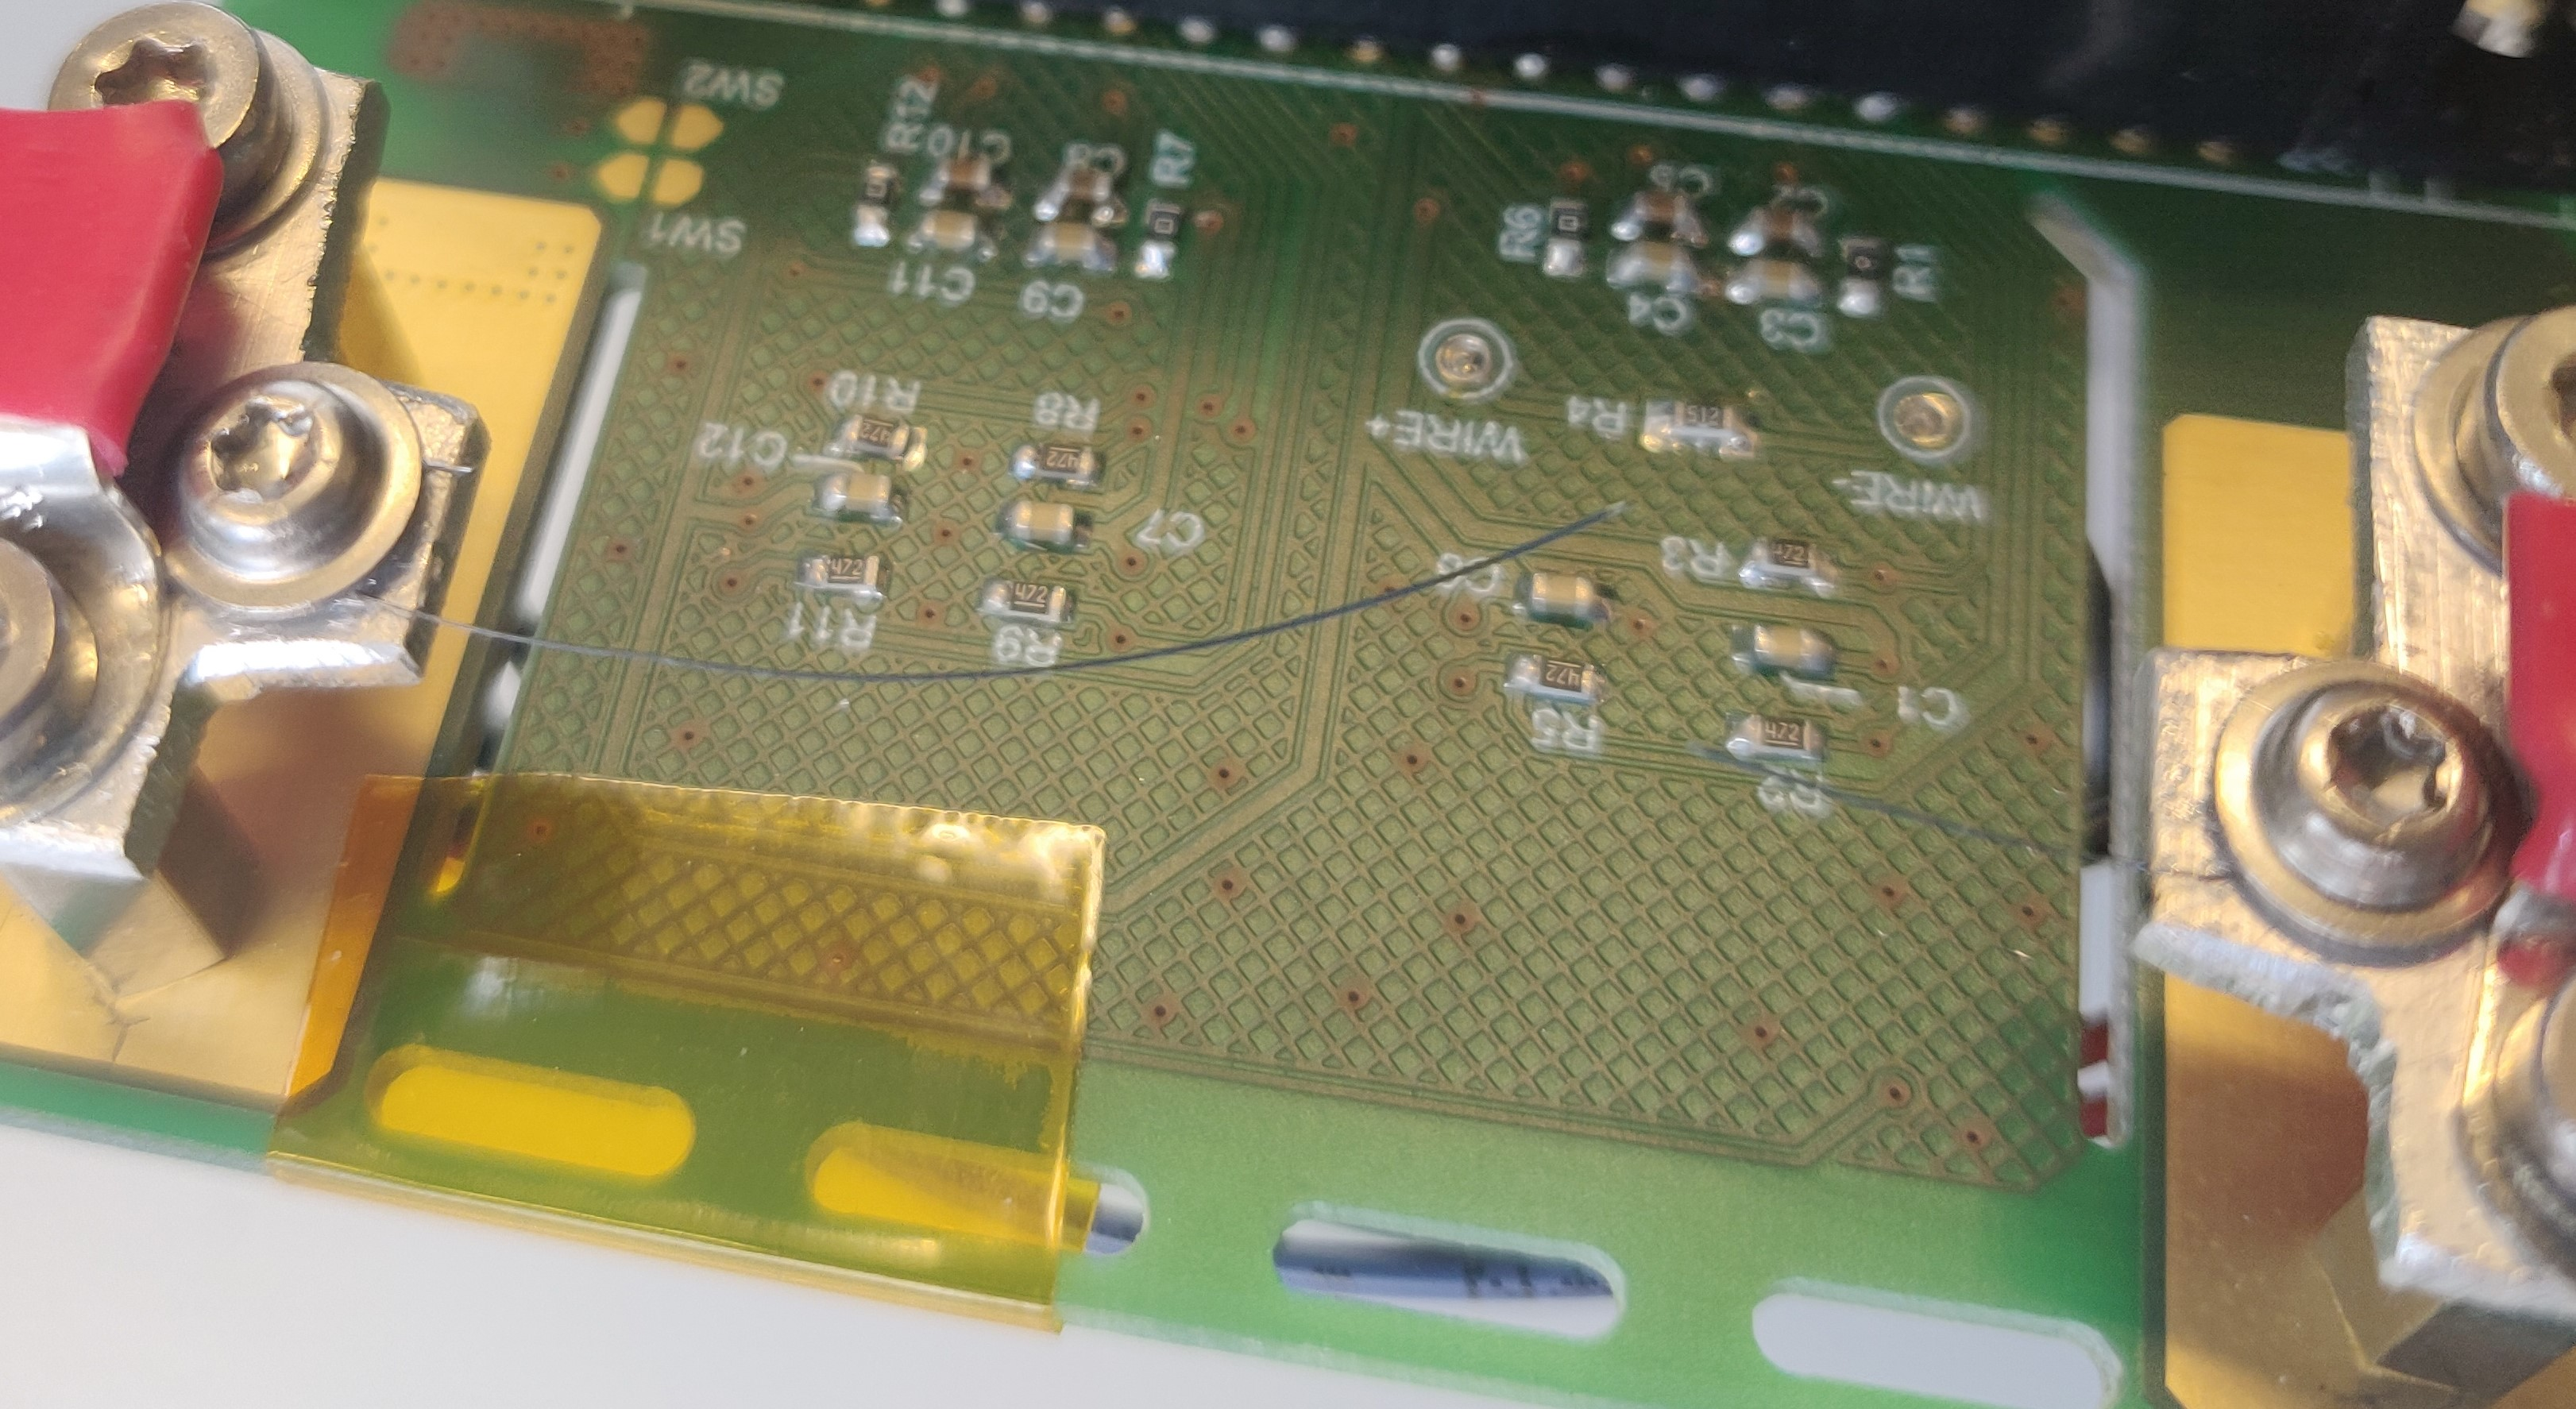
\includegraphics[width=0.7\columnwidth]{Figure_ColorChange/PictureWire.jpg}
    \caption{Tungsten wire after the measurements. Clear change of color is appreciated}
    \label{fig:Oxidation}
\end{figure}

\subsection{Transient State study}

For our analysis we were interested in the studitying the steady state of the system. But the implemented electronics were capable of also measuring the transient state to a maximum rate of $10^{4}$ samples per second. Figure \ref{fig:ResistanceWithTime} shows some more examples of the evolution of the resistance with time for three different applied currents. The transient state could be fitted by the following expression: 

\begin{equation}
    \Delta R (t) = A\cdot \left( 1 - \frac{1}{B e^{ \left( Ct \right)}}\right)
    \label{eq:Rt}
\end{equation}

Where A, B and C are constants obtained from the fit. This model seemed to fit very well the resistance variation when small currents were applied ($I < 100 mA$). The larger the intensity applied to the wire, the faster the system reaches the steady state. Figure \ref{fig:EvolParWithInt} shows how the time constant (C) changed as the intensity applied to the wire increased. Also in this picture we can observe how the relative error of the fitted curved varied with the increasing current. All these plots correspond to 40 $\mu m$ gold coated tungsten wires, but the behaviour was the same for the other samples. 

\begin{figure}[h]
    \centering
    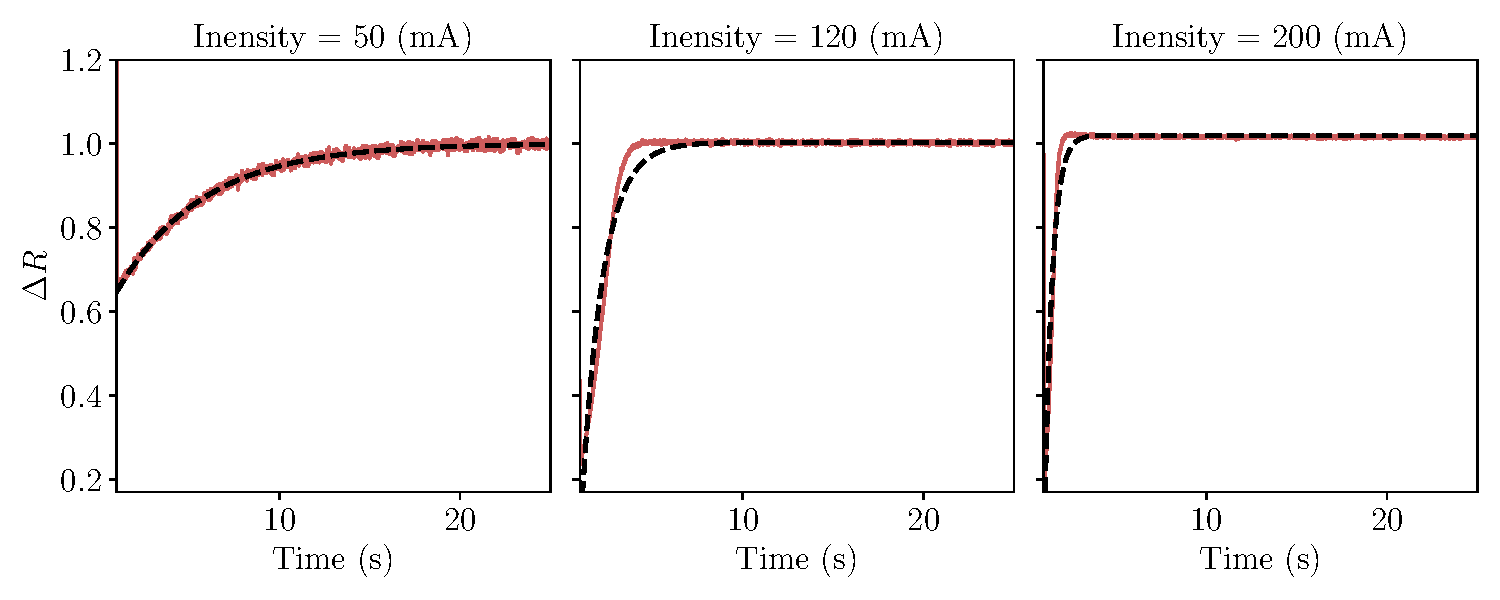
\includegraphics[width=1.0\columnwidth]{Figure_DeltaResTime/DeltaResTime.pdf}
    \caption{Variation of the resistance as a function of time for three different intensities applied to the wire. }
    \label{fig:ResistanceWithTime}
\end{figure}

\begin{figure}[h]
    \centering
    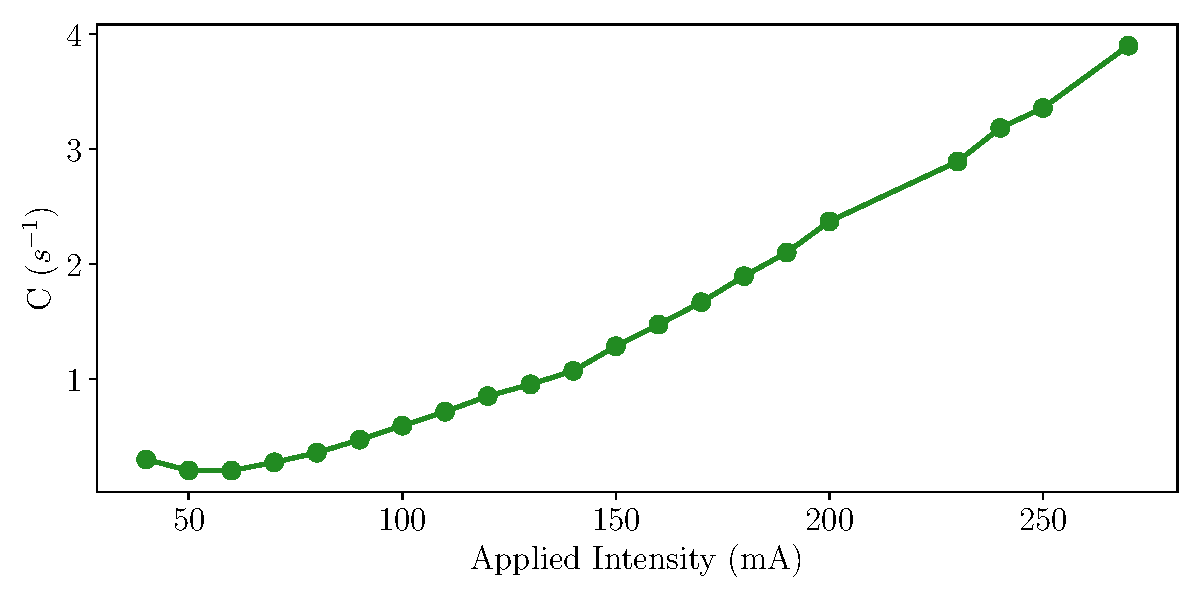
\includegraphics[width=0.7\columnwidth]{Figure_DeltaResTime/ParamEvolution.pdf}
    \caption{Evolution of time constant parameter (C) in equation \ref{eq:Rt} }
    \label{fig:EvolParWithInt}
\end{figure}



 
